% !TeX program = xelatex
% =====================================================================
% 数理统计课程论文 · 完整 LaTeX 主文件
% 论文标题：深度神经网络置信度校准的极大似然推断与假设检验：
%           基于 Temperature Scaling 的统计建模与实证分析
% 编译命令：xelatex -interaction=nonstopmode -enable-installer main.tex
% =====================================================================
\documentclass[a4paper,fontset=windows,zihao=-4]{ctexart}

% ---- 页面边距与行间距 ------------------------------------------------
\usepackage[a4paper,margin=2.54cm]{geometry}   % A4 纸张，标准四边 2.54cm
\usepackage{setspace}                          % 1.25 倍行距
\setstretch{1.25}

% ---- 数学公式、定理与符号宏包 ----------------------------------------
\usepackage{amsmath,amssymb}
\usepackage{amsthm}
\usepackage{mathtools}

% ---- 学术表格宏包 ----------------------------------------------------
\usepackage{booktabs}                          % 标准学术三线表
\usepackage{tabularx}                          % 自适应宽度表格
\usepackage{multirow}                          % 多行单元格合并
\usepackage{siunitx}                           % 科学计数与小数点列对齐

% ---- 图形与子图宏包 --------------------------------------------------
\usepackage{graphicx}
\usepackage{caption}
\usepackage{subcaption}
\graphicspath{{figures/}{../figures_calib/}{figures_calib/}}

% ---- 算法伪代码宏包 --------------------------------------------------
\usepackage[ruled,linesnumbered]{algorithm2e}
\SetAlgorithmName{算法}{算法}{算法清单}

% ---- 辅助工具宏包 ----------------------------------------------------
\usepackage{xcolor}
\usepackage{etoolbox}
\setmonofont{DejaVu Sans Mono}

% ---- 定理类环境声明 --------------------------------------------------
\newtheorem{prop}{命题}
\newtheorem{assumption}{假设}
\newtheorem{thm}{定理}
\newtheorem{defn}{定义}

% ---- 摘要页关键词宏 --------------------------------------------------
\newcommand{\keywords}[1]{\par\vspace{1.2em}\noindent{\heiti 关键词：}#1\par}

% ---- 浮动体排版优化参数 ----------------------------------------------
\renewcommand{\topfraction}{0.85}
\renewcommand{\floatpagefraction}{0.75}

% ---- 参考文献标题补丁（由 sec-refs.tex 独立控制 \section*{参考文献}）
\patchcmd{\thebibliography}{\section*{\refname}}{}{}%
  {\renewcommand{\refname}{}\PackageWarning{main}{patch of thebibliography heading failed; fell back to empty \refname}}

% ---- 超链接配置（最后加载）------------------------------------------
\usepackage[hidelinks]{hyperref}
\hypersetup{
  bookmarksnumbered,
  bookmarksdepth=2,
  pdftitle={深度神经网络置信度校准的极大似然推断与假设检验：基于 Temperature Scaling 的统计建模与实证分析},
  pdfauthor={数理统计课题组}
}

\begin{document}

% 封面页（仿《数理统计.pdf》第 1 页规范重建，无页码，不进目录）
% =====================================================================
% cover.tex — 封面页（无 \section，不进目录，无页码）
% 模板：数理统计.pdf 第 1 页规范重建
% =====================================================================
\thispagestyle{empty}
\newcommand{\coverline}[1]{%
  \rlap{\rule[-2.2pt]{240pt}{1.08pt}}\makebox[240pt][c]{\zihao{5}#1}}
\vspace*{1.83cm}
\begin{center}
  {\heiti\zihao{0}数理统计课程论文\par}
  \vspace{0.9cm}
  
\includegraphics[width=5.08cm]{hfut_logo}\par
  \vspace{1.4cm}
  {\songti\zihao{3}%
    \makebox[48bp][l]{题目：}%
    \begin{tabular}[c]{@{}c@{}}
      \coverline{深度神经网络置信度校准的极大似然推断与}\\[11pt]
      \coverline{假设检验：基于 Temperature Scaling 的}\\[11pt]
      \coverline{统计建模与实证分析}
    \end{tabular}\par}
  \vspace{0.6cm}
  {\songti\zihao{3}\makebox[48bp][l]{姓名：}\coverline{}}\par
  \vspace{1.55cm}
  {\songti\zihao{3}\makebox[48bp][l]{学号：}\coverline{}}\par
  \vspace{1.55cm}
  {\songti\zihao{3}\makebox[48bp][l]{学院：}\coverline{}}\par
\end{center}
\vfill
\begin{center}
  {\songti\zihao{3}2026-11-16\par}
\end{center}
\clearpage


% 摘要与关键词页（独立编号，从第 1 页起）
\clearpage
\pagestyle{plain}
\setcounter{page}{1}
% =====================================================================
% sec-abstract.tex — 摘要与关键词
% =====================================================================
\phantomsection
\addcontentsline{toc}{section}{摘要}
\begin{center}
  {\heiti\zihao{3} 摘\quad 要}
\end{center}
\vspace{0.5em}

现代深度分类神经网络在医疗诊断与自动驾驶等高风险决策场景中广泛应用，然而其预测概率普遍存在严重的「过度自信」现象，导致模型输出的高置信度无法真实反映预测正确的实际概率，削弱了决策系统的统计可靠性。为对这一概率失配问题进行严密的数理统计推断，本文将多分类 Softmax 后处理校准方法 Temperature Scaling 形式化纳入广义线性模型与极大似然估计（MLE）框架，旨在检验深度网络是否存在统计显著的校准偏差并构建完整的推断与检验体系。在理论层面，本文推导了逆温度参数 $\beta = 1/T$ 的对数似然函数、解析 Score 函数与观测 Fisher 信息量，通过条件方差非负性证明了似然函数的严格凹性与参数解的全局唯一性，并采用带回溯线搜索的阻尼 Newton--Raphson 迭代法进行数值求解；进一步借助一阶 Delta 方法推导了温度估计 $\hat T$ 的渐近方差并构造渐近置信区间，辅以非参数 Bootstrap 进行有限样本精度对照；构建了针对无需校准原假设 $H_0: T=1$ 的 Wald、Score 与似然比（LRT）三大渐近检验，并引入双参数 Platt Scaling 作为对照模型。在实证层面，基于 CIFAR-10 官方测试集（$N=10{,}000$ 样本，按 $2{,}000:8{,}000$ 分层划分为校准集与独立评估集，随机种子固定为 20261111），ResNet-20 与 ResNet-56 的温度估计分别为 $\hat T = 1.6245$（95\% Delta CI $[1.5147, 1.7343]$）与 $\hat T = 1.6904$（$[1.5884, 1.7925]$）；三大检验统计量均在 $p < 10^{-16}$ 显著性水平下拒绝原假设；在独立评估集上，两模型的期望校准误差（ECE）分别下降 $66.1\%$ 与 $68.6\%$，对数损失（NLL）分别降低 $17.7\%$ 与 $24.7\%$，Brier 分数显著改善（配对 Wilcoxon 检验 $p < 10^{-16}$，配对 $t$ 检验 $p < 10^{-14}$），且 McNemar 检验证实 Top-1 分类准确率保持不变（$p = 1.000$）。实证结果确证了极大似然估计满足理论 $O(n^{-1/2})$ 渐近相合速率，阐明了三大检验统计量经验排序的曲率机理，表明单参数 Temperature Scaling 在保持判别精度的前提下兼具良好的统计推断效能与实用性。

\keywords{置信度校准；极大似然估计；似然比检验；Delta 方法；Temperature Scaling}


% 目录页（两级目录）
\clearpage
\tableofcontents

% 正文主体部分
\clearpage
% =====================================================================
% sec-intro.tex — 第 1 节 引言
% 1.1 研究背景与科学问题界定
% 1.2 国内外研究现状综述（双脉络文献演进与既有研究统计缺口）
% 1.3 研究目标与主要工作
% 1.4 论文结构安排
% =====================================================================
\section{引言}\label{sec:intro}

\subsection{研究背景与科学问题界定}

随着深度神经网络在计算机视觉、自然语言处理等关键领域的突破性进展，深度学习模型已被广泛部署于医疗辅助诊断、自动驾驶避障决策、金融高频风控及司法量刑辅助等一系列安全攸关（Safety-Critical）的高风险现实场景中。在这些高风险决策体系中，算法系统所面临的核心诉求不仅局限于提供具有高判别精度的离散预测类别 $\hat Y \in \{1, \dots, C\}$，更为关键的是要求模型输出的后验预测概率向量 $\hat{\boldsymbol{p}} = (\hat p_1, \dots, \hat p_C)^\top$ 具备高度可靠的不确定性度量能力。

从数理统计的严格视角来看，预测概率的可靠性体现为统计\textbf{条件概率校准性}（Conditional Calibration）。形式化地，设输入特征空间为 $\mathcal{X} \subset \mathbb{R}^d$，真实类别标签空间为 $\mathcal{Y} = \{1, \dots, C\}$，其联合概率测度记为 $P(X, Y)$。对于任意给定的分类模型，记其离散预测标签为 $\hat Y(X) = \operatorname{argmax}_{c \in \{1,\dots,C\}} \hat p_c(X)$，所对应的最大预测置信度为 $\hat P(X) = \max_{c \in \{1,\dots,C\}} \hat p_c(X) \in [1/C, 1]$。若对于所有可能的置信度水平 $p \in [0, 1]$，真实类别的后验发生概率与模型输出的预测置信度严格相等，即满足：
\begin{equation}\label{eq:strong_calib_intro}
\mathbb{P}\big(Y = \hat Y(X) \;\big|\; \hat P(X) = p\big) = p, \quad \forall p \in [0, 1],
\end{equation}
则称该模型在置信度意义下满足严格条件概率校准。若式~\eqref{eq:strong_calib_intro}成立，则当模型以 $95\%$ 的置信度预测某批样本为特定类别时，该批样本中恰有 $95\%$ 为分类正确，下游决策引擎即可据此设定最优拒绝推断阈值或风险对冲策略。

然而，现代深度学习的发展却伴随着这一概率度量能力的系统性退化。自残差网络（ResNet）、批归一化（Batch Normalization）及大容量卷积架构普及以来，尽管模型在各类基准测试上的 Top-1 错误率被不断刷新，但输出概率却呈现出普遍而严重的「过度自信」（Overconfidence）倾向。在经验交叉熵损失函数的持续驱动下，梯度下降优化算法在模型分类准确率饱和后，仍会持续驱使输出对数几率（Logits）的模长不断增大，进而导致 Softmax 函数将预测概率极化推向概率单纯形的极角（多数样本置信度集中于 $0.95$ 以上）。尤为严峻的是，当深层网络做出错误决策时，其平均输出置信度仍往往高达 $80\%$ 甚至更高，形成严重的「虚假高确信」现象。

从统计推断的理论视角来看，过度自信在数学上表现为深度模型参数化输出分布与经验真实条件分布的系统性偏差。针对这一科学问题，学术界提出了以后处理方式缩放 logits 向量模长的 Temperature Scaling 方法。然而，该方法是否在数理统计意义上具备严密的参数估计基础？其温度估计量是否具有良好的渐近性质？如何构建规范的假设检验体系以判定网络是否显著偏离校准状态？网络容量深度对校准程度与统计推断结构有何内在影响？这些关键问题构成了本项研究探索的核心科学议题。

\subsection{国内外研究现状综述}

围绕分类模型的概率校准与不确定性评估，统计学界与机器学习界历经数十年的交叉演进，形成了两条层次鲜明的理论与方法脉络。

\textbf{脉络一：统计适当评分规则与经典概率校准理论。}
概率预测评估的理论基石源于气象统计与贝叶斯推断中关于「适当评分规则」（Proper Scoring Rules）的经典研究。Brier~\cite{brier1950verification} 首先提出了基于均方误差度量的 Brier Score，开启了概率预测准确性定量检验的先河。此后，Gneiting 与 Raftery~\cite{gneiting2007strictly} 在《美国统计学会会刊》（\textit{JASA}）上发表系统性综述，确立了严格适当评分规则（Strictly Proper Scoring Rules）的公理化数学框架，在测度论层面严格证明了：对数似然损失（Negative Log-Likelihood, NLL）与 Brier Score 的期望泛函取得全局极小值，当且仅当模型的预测条件分布与真实数据生成分布完全一致。该定理从数理统计底层证明了优化似然函数等价于追求最优概率校准。在传统统计学习中，针对支持向量机（SVM）等非概率边际分类器，Platt~\cite{platt1999probabilistic} 提出了基于二项似然的单变量双参数 Logistic 校准模型（即经典的 Platt Scaling）。随后，Zadrozny 与 Elkan~\cite{zadrozny2002transforming} 进一步引入了基于保序回归（Isotonic Regression）的非参数单调校准算法及直方图分箱映射，确立了经典机器学习后处理校准的基本范式。

\textbf{脉络二：现代深度神经网络的校准偏差与缩放校准方法。}
伴随着现代深度神经网络在参数深度与宽度上的大幅扩张，经典校准假设遭遇了显著挑战。Guo 等~\cite{guo2017calibration} 在国际机器学习大会（\textit{ICML}）上系统报告了现代深层网络的校准偏差现象：与早期的浅层多层感知机（MLP）或支持向量机相比，现代深层网络（如 ResNet、DenseNet）虽然判别精度大幅提高，但其条件校准误差却发生了系统性恶化，呈现出显著的过度自信；为此，他们提出了引入标量温度 $T$ 的 Temperature Scaling 后处理方案，在经验评估中展示了良好的分箱误差压缩效果。随后，Vaicenavicius 等~\cite{vaicenavicius2019evaluating} 从多变量分布检验视角探讨了连续校准误差度量的统计假设检验与核方法扩展；Minderer 等~\cite{minderer2021revisiting} 则在 \textit{NeurIPS} 上系统考察了视觉 Transformer（ViT）与卷积模型在跨领域分布偏移下的校准漂移现象，指出模型架构与训练目标对不确定性度量具有决定性约束。

\textbf{既有研究的统计推断缺口。}
综观既有文献，尽管以 Guo 等为代表的现代机器学习研究广泛应用了 Temperature Scaling，但绝大多数工作仍将其视作经验性的后处理超参数调优，尚缺乏系统性的数理统计学理论分析。具体表现在：
\begin{enumerate}
\item 鲜有文献从指数族极大似然估计角度，对温度参数（或其倒数逆温度 $\beta=1/T$）的对数似然严格凹性、解析 Score 方程与 Fisher 信息矩阵给出完备的数学证明，缺乏对估计解全局唯一存在性的理论保证；
\item 缺少基于大样本渐近理论（Asymptotic Normality）与 Delta 方法对温度参数估计量 $\hat T$ 渐近方差的解析推导，缺乏与非参数 Bootstrap 的有限样本区间覆盖对比；
\item 缺乏针对「网络是否需要校准」这一核心命题（即原假设 $H_0: T=1$）的形式化假设检验体系（Wald 检验、Score 检验与似然比检验 LRT），缺少对有限样本下三大检验统计量因似然曲率变化导致数值排序差异的数理阐释；
\item 缺乏结合网络深度对比验证估计量 $\sqrt{n}$ 渐近相合速率与有限总体修正（FPC）机制的精细实证支撑。
\end{enumerate}
针对上述学术空白，本文旨在将 Temperature Scaling 全面纳入经典数理统计理论体系，通过严谨的公式推导、渐近分析与无泄漏对照实验，构建一套完整的极大似然推断与假设检验分析框架。

\subsection{研究目标与主要工作}

本文以现代残差网络架构在标准 CIFAR-10 图像分类任务上的后验概率为实证载体，以浅层 ResNet-20（20 层，0.27M 参数）与深层 ResNet-56（56 层，0.85M 参数）为对照实体，将经典的数理统计推断与假设检验理论系统应用于已有的概率校准方法，并开展无泄漏实证对比分析。本文的主要工作概括如下：

\begin{enumerate}
\item \textbf{已有校准模型的指数族似然整理与 Lean 4 形式化核验}：针对 Guo 等~\cite{guo2017calibration} 提出的单参数 Temperature Scaling 方法，将其整理表达为多分类 Softmax 指数族条件似然模型，显式写出其一阶 Score 函数与二阶观测 Fisher 信息量（即类别 logit 的条件方差之和），阐明似然函数的严格凹性与 MLE 解的唯一存在性，采用标准的阻尼 Newton--Raphson 迭代法进行数值求解，并将上述核心推导在 Lean 4（Mathlib）环境下完成了机器形式化证明。
\item \textbf{经典渐近推断与统计假设检验方法的系统应用}：应用经典大样本渐近理论~\cite{lehmann1998theory,vandervaart1998asymptotic}、一阶 Delta 方法与非参数 Bootstrap~\cite{efron1994introduction}，计算温度估计量 $\hat T$ 的渐近方差与三类置信区间（Wald 区间、单调逆变换反演区间及 Bootstrap 百分位区间）；应用经典的 Wald、Score 与 LRT 检验对 $H_0: T=1$ 进行统计显著性裁决，并结合 Platt~\cite{platt1999probabilistic} 提出的双参数 Platt Scaling 对照，利用 McNemar 检验实证比较两类方法的准确率保序性。
\item \textbf{基于无泄漏协议的实证对比与跨模型深度效应分析}：在 CIFAR-10 官方测试集上采用分层无泄漏切分方案（$2{,}000:8{,}000$），完成 ResNet-20 与 ResNet-56 的独立实验与统计检验；在 $p < 10^{-16}$ 的显著性水平下证实了两类残差网络的过度自信现象，揭示了深层网络（ResNet-56, $\hat T=1.6904$）相比浅层网络（ResNet-20, $\hat T=1.6245$）更为显著的校准需求，并在独立评估集上实现了 ECE 下降超过 $66\%$ 的校准改善。
\item \textbf{有限样本实证现象的统计机理解释}：利用已有统计理论对实验中观察到的现象作出解释：用原假设点与 MLE 估计点处的局部 Fisher 信息差异（$I_n(1) \ll I_n(\hat\beta)$）解释三大检验统计量 $\text{Score} > \text{Wald} > \text{LRT}$ 的经验排序；借助抽样理论中的有限总体修正（FPC）公式解释样本量扩增下经验标准差略低于超总体 Delta 理论标准误的成因；并通过双对数线性回归验证了估计量满足经典 $O(n^{-1/2})$ 渐近相合速率。
\end{enumerate}

\subsection{论文结构安排}

全文共分为四个主体部分：
第~\ref{sec:intro} 节界定概率校准的科学问题，梳理国内外学术文献脉络并确立本文研究目标；
第~\ref{sec:theory} 节建立 Temperature Scaling 与 Platt Scaling 的统计模型设定，推导极大似然估计、Score 方程与二阶 Fisher 信息量，证明对数似然严格凹性，并构建 Delta 渐近推断与假设检验体系；
第~\ref{sec:empirical} 节详细介绍无泄漏实验设计、预处理与描述统计，围绕图~\ref{fig:fig1_eda} 至图~\ref{fig:fig5_convergence} 展开探索性数据分析、参数推断、综合评估及渐近理论的实证检验；
第~\ref{sec:discussion} 节深入剖析深度效应传导机制、三大检验排序成因、有限总体修正效应以及单双参数保序权衡，指出研究局限并给出标准化评测建议；
文末附有规范的 GB/T 7714 参考文献著录及附录。

% =====================================================================
% sec-theory-a.tex — 第 2 节 理论与方法基础（前半部）
% 2.1 概率校准的形式化定义与模型设定（TS 单参数模型与 Platt 双参数对照模型）
% 2.2 极大似然估计、Score 方程解析推导、Fisher 信息量与严格凹性数学证明
% =====================================================================
\section{理论与方法基础}\label{sec:theory}

\subsection{概率校准的形式化定义与模型设定}

在多分类机器学习与统计模式识别框架下，设样本观测值由多元随机向量 $X \in \mathcal{X} \subset \mathbb{R}^d$ 与真实离散类别标签 $Y \in \mathcal{Y} = \{1, 2, \dots, C\}$ 构成，其联合概率测度服从未知总体分布 $P(X, Y)$。深度分类模型的前向推理网络可形式化为一个可微参数映射 $f: \mathcal{X} \to \mathbb{R}^C$。对于输入特征向量 $X_i$，网络在最终线性分类层输出未经归一化的实值对数几率（Logit）向量：
\begin{equation}\label{eq:logit_vector}
\boldsymbol{z}_i = f(X_i) = \big(z_{i1}, z_{i2}, \dots, z_{iC}\big)^\top \in \mathbb{R}^C.
\end{equation}

在经典标准架构中，模型输出概率采用标准 Softmax 激活函数进行映射，得到经验后验预测分布向量 $\hat{\boldsymbol{p}}_i = (\hat p_{i1}, \dots, \hat p_{iC})^\top$：
\begin{equation}\label{eq:standard_softmax}
\hat p_{ic} = \frac{\exp(z_{ic})}{\sum_{k=1}^C \exp(z_{ik})}, \quad c = 1, 2, \dots, C.
\end{equation}
离散分类判决依据贝叶斯最大后验概率（MAP）准则给出：
\begin{equation}\label{eq:map_decision}
\hat Y_i = \operatorname{argmax}_{c \in \{1,\dots,C\}} \hat p_{ic} = \operatorname{argmax}_{c \in \{1,\dots,C\}} z_{ic},
\end{equation}
对应的最大预测置信度记为 $\hat P_i = \max_{c} \hat p_{ic} = \hat p_{i, \hat Y_i} \in [1/C, 1]$。

\begin{defn}[条件概率校准性]\label{defn:calibration}
若对于任意给定的概率预测水平 $p \in [0, 1]$，真实标签与模型判决类别一致的条件概率精确恒等于该预测概率水平，即：
\begin{equation}\label{eq:calibration_formal}
\mathbb{P}\big(Y = \hat Y \;\big|\; \hat P = p\big) = p, \quad \forall p \in [0, 1],
\end{equation}
则称该多分类模型满足严格条件概率校准。
\end{defn}

然而，在由大量卷积层与残差连接构成的现代网络中，经验损失最小化训练导致对数几率向量 $\boldsymbol{z}_i$ 的模长显著过大，打破了式~\eqref{eq:calibration_formal}的平衡，导致系统性的过度自信。为消除这一概率失配，我们建立后处理参数校准统计模型。

\subsubsection{单参数 Temperature Scaling 模型设定}

Temperature Scaling（温度缩放，TS）是一种作用于网络最终对数几率向量的多分类单参数后处理变换。本文将其形式化为单参数指数族分布。引入非负连续温度标量参数 $T \in (0, \infty)$，或等价引入其代数倒数——\textbf{逆温度参数}（Inverse Temperature Parameter）$\beta \equiv 1/T \in (0, \infty)$。给定样本 $i$ 的对数几率向量 $\boldsymbol{z}_i$，校准后的模型条件后验概率分布定义为：
\begin{equation}\label{eq:ts_model}
\begin{split}
p_{ic}(\beta) \equiv \mathbb{P}(Y_i = c \mid \boldsymbol{z}_i; \beta) &= \frac{\exp(\beta z_{ic})}{\sum_{k=1}^C \exp(\beta z_{ik})} \\
&= \operatorname{Softmax}_c(\beta \boldsymbol{z}_i), \quad c = 1, 2, \dots, C.
\end{split}
\end{equation}

单参数 Temperature Scaling 具有两个至关重要的数理统计特征：
\begin{prop}[严格保序性（Monotonic Order Preservation）]\label{prop:order_preservation}
对于任意给定的有限常数 $\beta \in (0, \infty)$ 以及任意样本对数几率分量，若存在两类别分量 $c, k \in \{1, \dots, C\}$ 满足 $z_{ic} > z_{ik}$，则当且仅当 $\beta > 0$ 时恒有：
\begin{equation}\label{eq:order_inequality}
p_{ic}(\beta) > p_{ik}(\beta).
\end{equation}
特别地，校准后的最大后验分类决策与未校准的原始网络决策严格恒等：
\begin{equation}\label{eq:argmax_invariance}
\operatorname{argmax}_{c \in \{1,\dots,C\}} p_{ic}(\beta) \equiv \operatorname{argmax}_{c \in \{1,\dots,C\}} z_{ic} \equiv \hat Y_i.
\end{equation}
\end{prop}

\begin{proof}
由指数函数的严格单调递增性，对任意 $\beta > 0$，有 $z_{ic} > z_{ik} \iff \beta z_{ic} > \beta z_{ik} \iff \exp(\beta z_{ic}) > \exp(\beta z_{ik})$。由于式~\eqref{eq:ts_model}中各分母归一化项 $\sum_k \exp(\beta z_{ik})$ 恒为严格正实数且与类别指标 $c$ 无关，两端同除分母不等号方向保持不变，即证式~\eqref{eq:order_inequality}。进而取极大值算子即可直接得出式~\eqref{eq:argmax_invariance}恒等成立。
\end{proof}

命题~\ref{prop:order_preservation}在理论上确立了 Temperature Scaling 的保序性质：\textbf{在后处理优化概率校准度的全过程中，模型的离散 Top-1 预测准确率在理论上保持不变，不会产生判别性能退化}。
从参数几何意义来看，当 $\beta = 1$（即 $T = 1$）时，模型精确退化为原始未校准网络；当 $\beta \in (0, 1)$（即 $T > 1$）时，$\beta$ 线性压缩了各类别 logit 之间的欧氏间距，使 Softmax 概率分布向中心平滑回缩，从而系统性抑制高置信度；当 $\beta \to 0$（即 $T \to \infty$）时，后验分布趋于离散均匀分布 $(1/C, \dots, 1/C)^\top$。

\subsubsection{双参数 Platt Scaling 对照模型设定}

为深入评估单参数缩放的简约性与相对优势，本文引入经典的双参数 Platt Scaling（Platt, 1999）作为基准对照模型。Platt Scaling 建立在模型 Top-1 预测的对数几率（Log-odds）标量变换之上。定义样本 $i$ 的标量预测几率为：
\begin{equation}\label{eq:log_odds}
x_i \equiv \operatorname{logit}(\hat P_i) = \log\left(\frac{\hat P_i}{1 - \hat P_i}\right) \in \mathbb{R}.
\end{equation}
在二项逻辑斯蒂回归（Logistic Regression）框架下，校准模型设定两个自由实数参数——偏置截距项 $\alpha \in \mathbb{R}$ 与斜率缩放项 $\beta_{\mathrm{platt}} \in \mathbb{R}$，重新估计 Top-1 类别预测为真实的概率 $q_i$：
\begin{equation}\label{eq:platt_formula}
\begin{split}
q_i(\alpha, \beta_{\mathrm{platt}}) &\equiv \mathbb{P}\big(Y_i = \hat Y_i \;\big|\; x_i; \alpha, \beta_{\mathrm{platt}}\big) \\
&= \sigma(\alpha + \beta_{\mathrm{platt}} x_i) = \frac{1}{1 + \exp\big(-(\alpha + \beta_{\mathrm{platt}} x_i)\big)},
\end{split}
\end{equation}
其中 $\sigma(\cdot)$ 为标准单变量 Sigmoid 激活函数。对于其余非 Top-1 类别的剩余概率，采用条件独立比例重归一化：
\begin{equation}\label{eq:platt_renorm}
\tilde p_{ic} = \frac{1 - q_i}{1 - \hat P_i} \hat p_{ic}, \quad \forall c \ne \hat Y_i.
\end{equation}

与单参数 Temperature Scaling 相比，Platt Scaling 引入了无约束的截距参数 $\alpha$。当 $\alpha \ne 0$ 时，校准映射不再通过原点，导致预测分类边界发生全局刚性平移。如果某样本的校准后概率满足 $q_i < 1/C$ 或引起非 Top-1 类别概率倒挂，则可能导致样本分类标签翻转，从而对模型的原始 Top-1 准确率造成外生性扰动。

\subsection{极大似然估计、Score 方程与严格凹性证明}

设有一组规模为 $n$ 的独立同分布（i.i.d.）校准数据集 $\mathcal{D}_{\mathrm{cal}} = \{(\boldsymbol{z}_i, y_i)\}_{i=1}^n$，其中 $\boldsymbol{z}_i \in \mathbb{R}^C$ 为预训练网络输出的对数几率向量，$y_i \in \{1, \dots, C\}$ 为真实的离散类别标签。引入独热（One-Hot）指示变量向量 $\boldsymbol{y}_i = (y_{i1}, \dots, y_{iC})^\top \in \{0, 1\}^C$，其中 $y_{ic} = \mathbf{1}(y_i = c)$。

\subsubsection{对数似然函数与解析 Score 方程}

在多分类指数族似然准则下，样本条件联合对数似然函数（Log-Likelihood Function）表示为逆温度参数 $\beta$ 的一元显式函数：
\begin{align}
\ell(\beta) &\equiv \sum_{i=1}^n \sum_{c=1}^C y_{ic} \log p_{ic}(\beta) \nonumber\\
&= \sum_{i=1}^n \sum_{c=1}^C y_{ic} \left[ \beta z_{ic} - \log \left( \sum_{k=1}^C \exp(\beta z_{ik}) \right) \right] \nonumber\\
&= \sum_{i=1}^n \left[ \beta z_{i, y_i} - \log \left( \sum_{k=1}^C \exp(\beta z_{ik}) \right) \right]. \label{eq:full_loglik}
\end{align}

对对数似然函数 $\ell(\beta)$ 关于参数 $\beta$ 求取一阶解析导数，可得统计学中的 \textbf{Score 函数}（记为 $U(\beta)$）：
\begin{align}
U(\beta) &\equiv \frac{\mathrm{d}\ell(\beta)}{\mathrm{d}\beta} = \sum_{i=1}^n \left[ z_{i, y_i} - \frac{\sum_{k=1}^C z_{ik} \exp(\beta z_{ik})}{\sum_{m=1}^C \exp(\beta z_{im})} \right] \nonumber\\
&= \sum_{i=1}^n \left[ z_{i, y_i} - \sum_{c=1}^C p_{ic}(\beta) z_{ic} \right]. \label{eq:score_derivation}
\end{align}

定义离散概率测度 $p_i(\beta)$ 下，样本 $i$ 处对数几率随机变量 $Z_i \in \{z_{i1}, \dots, z_{iC}\}$ 的条件期望为：
\begin{equation}\label{eq:conditional_expectation}
\mathbb{E}_{p_i(\beta)}[Z_i] \equiv \sum_{c=1}^C p_{ic}(\beta) z_{ic}.
\end{equation}
则 Score 函数式~\eqref{eq:score_derivation}可改写为真实观测值与模型期望值的残差和：
\begin{equation}\label{eq:score_clean}
U(\beta) = \sum_{i=1}^n \Big( z_{i, y_i} - \mathbb{E}_{p_i(\beta)}[Z_i] \Big).
\end{equation}
极大似然估计方程（Likelihood Equation）要求置 Score 函数为零，即 $U(\hat\beta) = 0$。该解析式表明：\textbf{在 MLE 估计点 $\hat\beta$ 处，全体校准样本中真实所属类别的 logit 总和等于在校准后模型分布测度下所计算的期望 logit 总和}。

\subsubsection{二阶导数、Fisher 信息量与严格凹性证明}

进一步对 Score 函数 $U(\beta)$ 求取关于参数 $\beta$ 的二阶导数。注意到 Softmax 概率关于 $\beta$ 的偏导数为：
\begin{equation}\label{eq:softmax_derivative}
\begin{split}
\frac{\mathrm{d} p_{ic}(\beta)}{\mathrm{d}\beta} &= p_{ic}(\beta) z_{ic} - p_{ic}(\beta) \left( \sum_{k=1}^C p_{ik}(\beta) z_{ik} \right) \\
&= p_{ic}(\beta) \big( z_{ic} - \mathbb{E}_{p_i(\beta)}[Z_i] \big).
\end{split}
\end{equation}
利用式~\eqref{eq:softmax_derivative}，直接对式~\eqref{eq:score_derivation}求导：
\begin{align}
\frac{\mathrm{d}^2\ell(\beta)}{\mathrm{d}\beta^2} &= \frac{\mathrm{d} U(\beta)}{\mathrm{d}\beta} = - \sum_{i=1}^n \sum_{c=1}^C z_{ic} \frac{\mathrm{d} p_{ic}(\beta)}{\mathrm{d}\beta} \nonumber\\
&= - \sum_{i=1}^n \sum_{c=1}^C z_{ic} \left[ p_{ic}(\beta) z_{ic} - p_{ic}(\beta) \sum_{k=1}^C p_{ik}(\beta) z_{ik} \right] \nonumber\\
&= - \sum_{i=1}^n \left[ \sum_{c=1}^C p_{ic}(\beta) z_{ic}^2 - \left( \sum_{c=1}^C p_{ic}(\beta) z_{ic} \right)^2 \right]. \label{eq:second_deriv}
\end{align}

根据数理统计理论，定义样本\textbf{观测 Fisher 信息量}（Observed Fisher Information）为负二阶导数：
\begin{equation}\label{eq:fisher_defn}
I_n(\beta) \equiv - \frac{\mathrm{d}^2\ell(\beta)}{\mathrm{d}\beta^2} = - \ell''(\beta).
\end{equation}
式~\eqref{eq:second_deriv}中方括号内的第二项为条件期望的平方，第一项为条件二阶矩 $\mathbb{E}_{p_i(\beta)}[Z_i^2] = \sum_{c=1}^C p_{ic}(\beta) z_{ic}^2$。因此，该方括号恒等于离散随机变量 $Z_i$ 在分布 $p_i(\beta)$ 下的\textbf{条件方差}（Conditional Variance）：
\begin{equation}\label{eq:fisher_variance}
I_n(\beta) = \sum_{i=1}^n \operatorname{Var}_{p_i(\beta)}(Z_i).
\end{equation}

基于式~\eqref{eq:fisher_variance}，我们给出本模型最核心的数学收敛性定理：

\begin{thm}[对数似然的严格凹性与 MLE 唯一全局最优性]\label{thm:strict_concavity}
设校准集 $\mathcal{D}_{\mathrm{cal}}$ 中至少存在一个样本 $i$，其输出对数几率向量是非退化的（即存在至少两类 $c \ne k$ 使得 $z_{ic} \ne z_{ik}$）。则对于任意参数值 $\beta \in (0, \infty)$，观测 Fisher 信息量严格正定：
\begin{equation}\label{eq:fisher_positive}
I_n(\beta) > 0, \quad \forall \beta \in (0, \infty).
\end{equation}
进而，对数似然函数 $\ell(\beta)$ 在开区间 $(0, \infty)$ 上处处严格凹（Strictly Concave）。若 Score 方程 $U(\beta) = 0$ 在定义域内存在实根，则极大似然估计解 $\hat\beta$ 全局唯一。
\end{thm}

\begin{proof}
根据概率论基本性质，对于任意非退化离散随机变量，其方差恒满足 $\operatorname{Var}(X) \ge 0$，且取等号当且仅当随机变量以概率 1 退化为常数。
对于任意样本 $i$ 以及任意有限参数 $\beta \in (0, \infty)$，由指数映射性质可知 Softmax 条件概率恒满足严格内点条件：$p_{ic}(\beta) \in (0, 1)$。由于假定存在样本 $i$ 使得类别间 logit 取值不完全相等，该样本对数几率在分布测度 $p_i(\beta)$ 下不退化为常数，因此该样本的条件方差严格大于零：
\[
\operatorname{Var}_{p_i(\beta)}(Z_i) > 0.
\]
将其代入式~\eqref{eq:fisher_variance}，作为非负项与至少一个严格正项的有限求和，必然得出：
\[
I_n(\beta) = \sum_{i=1}^n \operatorname{Var}_{p_i(\beta)}(Z_i) > 0, \quad \forall \beta \in (0, \infty).
\]
从而对数似然的二阶导数处处严格为负：
\[
\ell''(\beta) = -I_n(\beta) < 0, \quad \forall \beta \in (0, \infty).
\]
由凸分析基本定理，定义在凸集上的二次连续可微函数若其二阶导数恒严格负，则该函数在该凸集上严格凹。若严格凹函数在开区间内部存在一阶导数为零的驻点 $\hat\beta$（即 $U(\hat\beta)=0$），则该点必为唯一的全局极大值点。定理证毕。
\end{proof}

\subsubsection{阻尼 Newton--Raphson 求解}

得益于定理~\ref{thm:strict_concavity}所保证的全局严格凹性，对数似然曲面上不存在局部非凸陷阱或伪驻点。此外，二阶导数式~\eqref{eq:fisher_variance}具备条件方差的闭式表达，便于采用二阶牛顿法高效求解。本文采用标准的带回溯线搜索（Backtracking Line Search）的阻尼 Newton--Raphson 迭代法求解 $\hat\beta$：
\begin{equation}\label{eq:newton_iteration}
\beta^{(t+1)} = \beta^{(t)} + \gamma_t \frac{U(\beta^{(t)})}{I_n(\beta^{(t)})}, \quad t = 0, 1, 2, \dots
\end{equation}
其中，初始点设为未校准状态 $\beta^{(0)} = 1.0$；$\gamma_t \in (0, 1]$ 为阻尼步长因子，初始设为 $1.0$。在每次迭代中，若试探步无法满足单调似然上升条件：
\begin{equation}\label{eq:armijo}
\ell\left(\beta^{(t)} + \gamma_t \frac{U(\beta^{(t)})}{I_n(\beta^{(t)})}\right) < \ell\left(\beta^{(t)}\right),
\end{equation}
则按比例收缩步长 $\gamma_t \leftarrow \gamma_t / 2$；同时对更新值施加保护截断 $\beta \ge 0.05$ 以防止边界发散。迭代收敛判据设定为连续两次更新步长的绝对变化量小于极小公差：$|\beta^{(t+1)} - \beta^{(t)}| < 10^{-12}$。在实测中，得益于二阶导数的精确解析性，该算法通常在 $8 \sim 15$ 次迭代内即可达成机器精度收敛。

% =====================================================================
% sec-theory-b.tex — 第 2 节 理论与方法基础（后半部）
% 2.3 渐近理论、Delta 方法与非参数 Bootstrap 置信区间构造
% 2.4 校准需求与校准效果的统计假设检验体系（原假设三大检验与评估集配对检验）
% =====================================================================

\subsection{渐近理论、Delta 方法与置信区间构造}

在数理统计推断中，点估计量 $\hat\beta$ 与 $\hat T$ 仅提供了有限样本下的经验最优解，唯有结合其抽样分布建立渐近理论并构造置信区间，方能对深度模型的真实过度自信程度进行量化的统计不确定性界定。

\subsubsection{极大似然估计的渐近正态性与 Wald 区间}

根据 Cramér--Rao 极大似然估计的经典大样本渐近理论~\cite{lehmann1998theory,vandervaart1998asymptotic}，在对数似然函数连续可微、支撑集与参数无关以及 Fisher 信息量正定等标准正则性条件满足的前提下，随着校准集样本容量 $n \to \infty$，无约束极大似然估计量 $\hat\beta$ 具有弱相合性与渐近有效性，并渐近收敛于一元高斯分布：
\begin{equation}\label{eq:asymptotic_beta}
\sqrt{n}\big(\hat\beta - \beta_0\big) \xrightarrow{d} \mathcal{N}\left(0, \;\mathcal{I}_1(\beta_0)^{-1}\right),
\end{equation}
其中 $\beta_0$ 为数据生成过程的真实参数值，$\mathcal{I}_1(\beta_0) \equiv \lim_{n \to \infty} \frac{1}{n} I_n(\beta_0)$ 为单样本期望 Fisher 信息量。

在实际有限样本推断中，真实参数 $\beta_0$ 未知，采用极大似然估计点处的观测 Fisher 信息量 $I_n(\hat\beta)$ 进行代换估计。由连续映射定理与 Slutsky 定理，$\hat\beta$ 的有限样本渐近方差估计量为：
\begin{equation}\label{eq:var_beta_est}
\widehat{\operatorname{Var}}(\hat\beta) = I_n(\hat\beta)^{-1} = \frac{1}{\sum_{i=1}^n \operatorname{Var}_{p_i(\hat\beta)}(Z_i)}.
\end{equation}
对应逆温度参数估计量 $\hat\beta$ 的渐近标准误（Standard Error, SE）显式表达为：
\begin{equation}\label{eq:se_beta}
\mathrm{SE}(\hat\beta) \equiv \sqrt{\widehat{\operatorname{Var}}(\hat\beta)} = \frac{1}{\sqrt{I_n(\hat\beta)}}.
\end{equation}
据此，对于任意置信水平 $1-\alpha \in (0, 1)$，参数 $\beta$ 的大样本渐近 Wald 双侧置信区间构造为：
\begin{equation}\label{eq:wald_ci_beta}
\begin{split}
\mathrm{CI}_{1-\alpha}(\beta) = \big[ &\hat\beta - z_{1-\alpha/2}\mathrm{SE}(\hat\beta), \\
&\hat\beta + z_{1-\alpha/2}\mathrm{SE}(\hat\beta) \big],
\end{split}
\end{equation}
其中 $z_{1-\alpha/2}$ 为标准正态分布的 $1-\alpha/2$ 分位数（取 $\alpha=0.05$ 时为 $1.95996 \approx 1.96$）。

\subsubsection{Delta 方法推导温度参数 $\hat T$ 的渐近方差}

在深度学习与置信度校准实践中，具有直观物理语义的参数是正温度标量 $T = 1/\beta$。然而，$\hat T \equiv 1/\hat\beta$ 是关于随机变量 $\hat\beta$ 的非线性代数变换。为解析导出 $\hat T$ 的极限抽样分布与标准误，需引入统计学中的 \textbf{Delta 方法}（Delta Method）。

定义单变量非线性光滑标量函数 $g: (0, \infty) \to (0, \infty)$ 为：
\begin{equation}\label{eq:g_transform}
g(\beta) \equiv \frac{1}{\beta}.
\end{equation}
函数 $g(\beta)$ 在开区间 $(0, \infty)$ 上处处一阶连续可微，其一阶导数函数为：
\begin{equation}\label{eq:g_prime}
g'(\beta) = - \frac{1}{\beta^2}.
\end{equation}

根据一元 Delta 方法的泰勒一阶展开定理，若序列满足 $\sqrt{n}(\hat\beta - \beta_0) \xrightarrow{d} \mathcal{N}(0, \sigma^2)$，且 $g'(\beta_0) \ne 0$，则变换后随机序列的渐近分布满足：
\begin{equation}\label{eq:delta_theorem}
\sqrt{n}\Big(g(\hat\beta) - g(\beta_0)\Big) \xrightarrow{d} \mathcal{N}\left(0, \;\big[g'(\beta_0)\big]^2 \sigma^2\right).
\end{equation}

将式~\eqref{eq:var_beta_est}与式~\eqref{eq:g_prime}代入定理式~\eqref{eq:delta_theorem}，温度估计量 $\hat T = g(\hat\beta)$ 的有限样本渐近方差可解析导出为：
\begin{align}
\widehat{\operatorname{Var}}(\hat T) &\approx \big[g'(\hat\beta)\big]^2 \widehat{\operatorname{Var}}(\hat\beta) \nonumber\\
&= \left( - \frac{1}{\hat\beta^2} \right)^2 \frac{1}{I_n(\hat\beta)} \nonumber\\
&= \frac{1}{\hat\beta^4 I_n(\hat\beta)} = \frac{\hat T^4}{I_n(\hat\beta)}. \label{eq:t_variance_analytic}
\end{align}

取方差的平方根，即可得到温度参数估计量 $\hat T$ 的一阶 Delta 渐近标准误（Delta Standard Error）：
\begin{equation}\label{eq:delta_se_formula}
\begin{split}
\mathrm{SE}_\Delta(\hat T) &= \frac{\mathrm{SE}(\hat\beta)}{\hat\beta^2} = \hat T^2 \mathrm{SE}(\hat\beta) \\
&= \frac{1}{\hat\beta^2 \sqrt{I_n(\hat\beta)}}.
\end{split}
\end{equation}
由此，温度参数 $T$ 在置信水平 $1-\alpha$（取 $95\%$）下的对称渐近 Wald 置信区间为：
\begin{equation}\label{eq:wald_ci_T}
\begin{split}
\mathrm{CI}_{\Delta, 1-\alpha}(T) = \big[ &\hat T - z_{1-\alpha/2} \mathrm{SE}_\Delta(\hat T), \\
&\hat T + z_{1-\alpha/2} \mathrm{SE}_\Delta(\hat T) \big].
\end{split}
\end{equation}

\subsubsection{单调逆变换反演区间与非参数 Bootstrap 百分位区间}

除一阶线性化 Wald 区间外，本文进一步构建两类精度更高的置信区间：

\textbf{1. 单调逆变换反演置信区间（Inversion Confidence Interval）。}
注意到变换函数 $g(\beta) = 1/\beta$ 在开区间 $(0, \infty)$ 上是严格单调递减的双射函数。若我们已知参数 $\beta$ 的 $1-\alpha$ 置信区间为 $[\beta_L, \beta_U] = [\hat\beta - z_{1-\alpha/2}\mathrm{SE}(\hat\beta), \; \hat\beta + z_{1-\alpha/2}\mathrm{SE}(\hat\beta)]$，则根据概率测度的保序性质：
\[
\mathbb{P}\big(\beta_L \le \beta \le \beta_U\big) = \mathbb{P}\left(\frac{1}{\beta_U} \le \frac{1}{\beta} \le \frac{1}{\beta_L}\right) = \mathbb{P}\left(\frac{1}{\beta_U} \le T \le \frac{1}{\beta_L}\right) = 1 - \alpha.
\]
由此导出的单调反演置信区间显式定义为：
\begin{equation}\label{eq:inversion_ci}
\begin{split}
\mathrm{CI}_{\mathrm{inv}, 1-\alpha}(T) \equiv \Bigg[ &\frac{1}{\hat\beta + z_{1-\alpha/2}\mathrm{SE}(\hat\beta)}, \\
&\frac{1}{\hat\beta - z_{1-\alpha/2}\mathrm{SE}(\hat\beta)} \Bigg].
\end{split}
\end{equation}
由于 $g(x) = 1/x$ 具有正二阶导数（严格凸性），反演区间天然具有非对称自适应调节能力，能够合理反映非线性变换带来的右偏几何特性，避免了 Wald 区间在极端参数下出现的负值或对称失真。

\textbf{2. 非参数 Bootstrap 百分位置信区间（Percentile Bootstrap CI）。}
为了在有限样本下摆脱渐近正态分布理论假设的束缚，评估经验抽样分布的稳健性，本文构建基于经验重抽样（Empirical Resampling）的非参数 Bootstrap 方法~\cite{efron1994introduction}：
\begin{enumerate}
\item 给定校准数据集 $\mathcal{D}_{\mathrm{cal}} = \{(\boldsymbol{z}_i, y_i)\}_{i=1}^n$；
\item 以均匀等概率进行有放回独立抽样 $n$ 次，构造第 $b$ 次重抽样样本集 $\mathcal{D}^*_b$（$b = 1, 2, \dots, B$，$B = 2000$）；
\item 在每个重抽样集 $\mathcal{D}^*_b$ 上，独立调用阻尼 Newton--Raphson 算法求解得到逆温度极大似然估计 $\hat\beta^*_b$，并计算温度重抽样估计量 $\hat T^*_b = 1/\hat\beta^*_b$；
\item 将 $B$ 个估计值按升序排列：$\hat T^*_{(1)} \le \hat T^*_{(2)} \le \dots \le \hat T^*_{(B)}$；
\item 取排序序列的经验分位数，构造 $95\%$ 非参数百分位置信区间：
\begin{equation}\label{eq:bootstrap_ci}
\mathrm{CI}_{\mathrm{boot}, 0.95}(T) = \left[ \hat T^*_{\big(\lfloor 0.025 B \rfloor\big)}, \; \hat T^*_{\big(\lceil 0.975 B \rceil\big)} \right].
\end{equation}
\end{enumerate}

\subsection{校准需求与校准效果的统计假设检验体系}

为从统计显著性层面严密裁定模型是否存在校准偏差，并科学评价校准带来的泛化性能增益，本文构建分层双轨检验体系：在参数层面建立针对无需校准原假设的三大经典渐近检验，在评估集层面建立针对预测损失与分类决策的多维非参数配对检验。

\subsubsection{模型校准需求的原假设检验体系（Wald / Score / LRT）}

在数理统计推断中，判定网络是否处于严格校准状态等价于判定温度参数是否显著偏离基准值 1.0。形式化地，建立如下双侧统计原假设与备择假设：
\begin{equation}\label{eq:null_hypothesis}
H_0: \beta = 1 \quad (\text{即 } T = 1, \text{ 模型无需校准}), \quad \text{vs.} \quad H_1: \beta \ne 1 \quad (\text{即 } T \ne 1).
\end{equation}

针对这一经典的复合参数检验问题，数理统计学三大基石检验方法均可在此构建闭式检验统计量：

\textbf{1. 瓦尔德检验（Wald Test）。}
Wald 检验基于无约束极大似然估计点 $\hat\beta$ 与受限原假设点 $\beta_0=1$ 之间的参数欧氏距离，并以 MLE 点处的观测 Fisher 信息量进行二次型加权：
\begin{equation}\label{eq:wald_test_stat}
W \equiv \big(\hat\beta - 1\big)^2 I_n(\hat\beta) = \frac{(\hat\beta - 1)^2}{\widehat{\operatorname{Var}}(\hat\beta)}.
\end{equation}
在原假设 $H_0$ 为真的条件下，由大样本渐近理论，统计量渐近服从自由度为 1 的卡方分布：
\begin{equation}\label{eq:wald_distribution}
W \xrightarrow{d} \chi^2_1.
\end{equation}

\textbf{2. 评分检验 / 拉奥检验（Score Test / Rao Test）。}
Score 检验的核心理论优势在于\textbf{无需求解备择假设下的无约束极大似然估计 $\hat\beta$}，仅需在受限原假设点 $\beta=1$ 处评估对数似然函数的一阶导数（梯度）与二阶曲率：
\begin{equation}\label{eq:score_test_stat}
\begin{split}
S &\equiv \frac{\big[U(1)\big]^2}{I_n(1)} \\
&= \frac{\left[ \sum_{i=1}^n \big( z_{i, y_i} - \mathbb{E}_{p_i(1)}[Z_i] \big) \right]^2}{\sum_{i=1}^n \operatorname{Var}_{p_i(1)}(Z_i)}.
\end{split}
\end{equation}
在原假设 $H_0$ 成立时，根据中心极限定理，$U(1)/\sqrt{I_n(1)} \xrightarrow{d} \mathcal{N}(0, 1)$，其平方统计量渐近服从卡方分布：
\begin{equation}\label{eq:score_distribution}
S \xrightarrow{d} \chi^2_1.
\end{equation}

\textbf{3. 似然比检验（Likelihood Ratio Test, LRT）。}
似然比检验直接衡量无约束最大对数似然值与原假设受限对数似然值之间的对数似然倍数增益：
\begin{equation}\label{eq:lrt_test_stat}
\Lambda \equiv 2 \big[ \ell(\hat\beta) - \ell(1) \big].
\end{equation}
由经典的 Wilks 定理，在原假设 $H_0$ 成立时，由于受限参数空间维数与全空间维数之差为 $1 - 0 = 1$，似然比统计量渐近服从自由度为 1 的卡方分布：
\begin{equation}\label{eq:lrt_distribution}
\Lambda \xrightarrow{d} \chi^2_1.
\end{equation}

在标准渐近理论中，当样本量 $n \to \infty$ 且真实参数邻近原假设时，Wald、Score 与 LRT 渐近等价。然而在深度神经网络显著过度自信的实证场景中，真实估计值 $\hat\beta \approx 0.6$ 与原假设 $\beta_0=1$ 相距甚远。此时，对数似然曲面呈现显著的非二次非对称性曲率，直接诱发三大统计量产生可预测的系统性数值差异（详见第~\ref{sec:discussion} 节讨论）。

\subsubsection{评估集多维校准指标与配对样本检验体系}

为了在独立的留出评估集 $\mathcal{D}_{\mathrm{eval}} = \{(\boldsymbol{z}_j, y_j)\}_{j=1}^{n_{\mathrm{eval}}}$（$n_{\mathrm{eval}}=8{,}000$）上全面衡量概率校准的实际效能，本文定义四项互补的统计度量指标：

\begin{enumerate}
\item \textbf{负对数似然损失（Negative Log-Likelihood, NLL）}：作为严格适当评分规则，衡量全概率分布与真实标签的交叉熵发散度：
\begin{equation}\label{eq:nll_eval}
\mathrm{NLL} \equiv - \frac{1}{n_{\mathrm{eval}}} \sum_{j=1}^{n_{\mathrm{eval}}} \log p_{j, y_j}(\hat\beta).
\end{equation}
\item \textbf{Brier 分数（Brier Score, BS）}：作为另一严格适当评分规则，度量预测概率向量与独热真实标签之间的欧氏均方距离：
\begin{equation}\label{eq:brier_eval}
\mathrm{BS} \equiv \frac{1}{n_{\mathrm{eval}}} \sum_{j=1}^{n_{\mathrm{eval}}} \sum_{c=1}^C \Big( p_{jc}(\hat\beta) - \mathbf{1}(y_j = c) \Big)^2.
\end{equation}
\item \textbf{期望校准误差（Expected Calibration Error, ECE）}：将置信度区间 $[0, 1]$ 划分为 $M$ 个等宽区间分箱 $B_m = (\frac{m-1}{M}, \frac{m}{M}]$，加权累加各分箱内预测置信度与实际分类经验准确率的绝对偏差：
\begin{equation}\label{eq:ece_eval}
\mathrm{ECE} \equiv \sum_{m=1}^M \frac{|B_m|}{n_{\mathrm{eval}}} \Big| \operatorname{acc}(B_m) - \operatorname{conf}(B_m) \Big|,
\end{equation}
其中 $\operatorname{acc}(B_m) = \frac{1}{|B_m|} \sum_{j \in B_m} \mathbf{1}(\hat Y_j = y_j)$，$\operatorname{conf}(B_m) = \frac{1}{|B_m|} \sum_{j \in B_m} \hat P_j$。
\item \textbf{最大校准误差（Maximum Calibration Error, MCE）}：衡量全部分箱中极端最差情况下的最大校准偏差：
\begin{equation}\label{eq:mce_eval}
\mathrm{MCE} \equiv \max_{m \in \{1, \dots, M\}} \Big| \operatorname{acc}(B_m) - \operatorname{conf}(B_m) \Big|.
\end{equation}
\end{enumerate}

在评估集的多维统计检验方面，为克服单一均值指标无法反映样本级微观变化的局限，构建如下检验：
\begin{itemize}
\item \textbf{样本级配对 Wilcoxon 符号秩检验与配对 $t$ 检验}：针对每个独立测试样本 $j$，计算校准前后的损失变化量 $\Delta \mathrm{BS}_j = \mathrm{BS}_j^{\mathrm{cal}} - \mathrm{BS}_j^{\mathrm{uncal}}$ 与 $\Delta \mathrm{NLL}_j = \mathrm{NLL}_j^{\mathrm{cal}} - \mathrm{NLL}_j^{\mathrm{uncal}}$（负值表示校准后损失降低）。构建原假设 $H_0: \mathbb{E}[\Delta] = 0$，通过配对 $t$ 检验与非参数 Wilcoxon 符号秩检验，判定校准带来的损失降低是否在全样本微观层面达到统计显著。
\item \textbf{McNemar 决策一致性列联表检验}：为核验校准对离散分类判决的影响，构建如下 $2 \times 2$ 分类正误列联表：
\begin{center}\small
\begin{tabular}{lcc}
\toprule
 & 校准后正确 & 校准后错误 \\
\midrule
未校准正确 & $a$ & $b$ \\
未校准错误 & $c$ & $d$ \\
\bottomrule
\end{tabular}
\end{center}
其中 $b$ 为未校准正确但校准后错误的样本数，$c$ 为未校准错误但校准后正确的样本数。连续性修正的 McNemar 检验统计量定义为：
\begin{equation}\label{eq:mcnemar_stat}
\chi^2_{\mathrm{McNemar}} =
\begin{cases}
\dfrac{\big(|b - c| - 1\big)^2}{b + c}, & b + c > 0 \text{ 且 } |b - c| \ge 1, \\[6pt]
0, & b + c = 0 \text{ 或 } |b - c| < 1.
\end{cases}
\end{equation}
当 $b + c \to \infty$ 时，在原假设 $H_0: p_b = p_c$ 下 $\chi^2_{\mathrm{McNemar}} \xrightarrow{d} \chi^2_1$。当两模型决策完全一致时，$b=0, c=0$，检验统计量为 $0.0$，$p$ 值为 $1.000$。这一检验将为对比单参数 Temperature Scaling 与双参数 Platt Scaling 的保序性能提供量化基准。
\end{itemize}

% =====================================================================
% sec-empirical.tex — 第 3 节 实例分析与实证结果
% 3.1 数据来源与无泄漏实验设计
% 3.2 数据预处理与基础描述统计（表 1）
% 3.3 过度自信特征的探索性数据分析（EDA，图 1）
% 3.4 模型求解、参数推断与假设检验结果（表 2、图 2、表 3）
% 3.5 校准效果可视化与渐近理论实证验证（图 3、图 4、图 5）
% =====================================================================
\section{实例分析与实证结果}\label{sec:empirical}

\subsection{数据来源与无泄漏实验设计}

为检验 Temperature Scaling 与 Platt Scaling 在实际图像模式识别系统中的统计推断性质，本文选取计算机视觉领域经典的 CIFAR-10 官方基准测试集作为实证载体。CIFAR-10 测试集共包含 $N = 10{,}000$ 张标准 $32 \times 32$ 像素的三通道彩色图像，严格均衡分布在 10 个互斥类别（飞机、汽车、鸟、猫、鹿、狗、青蛙、马、船、卡车）中，每个类别精确包含 1,000 张图像。

在分类模型方面，本文选取具有代表性深度的两种残差网络架构：
\begin{enumerate}
\item \textbf{ResNet-20}：代表浅层现代卷积网络，包含 20 个加权卷积层，总参数量约为 0.27M；
\item \textbf{ResNet-56}：代表深层现代卷积网络，包含 56 个加权卷积层，总参数量约为 0.85M（参数规模约为 ResNet-20 的 3.15 倍）。
\end{enumerate}
两模型权重均采用 PyTorch 官方基准仓库（\texttt{chenyaofo/pytorch-cifar-models}）的公开预训练权重，且模型在训练阶段仅接触 CIFAR-10 训练集（50,000 张图像），官方测试集的 10,000 张图像在模型训练与特征学习阶段完全隔离，保证了特征提取的客观性。

在数理统计校准实验中，严防数据泄漏（Data Leakage）是保障统计推断有效性与泛化评估无偏性的根本前提。若在拟合校准参数的样本上评估校准误差，会导致乐观偏误。为此，本文设计了\textbf{分层抽样独立划分方案}（Stratified Shuffle Split）：
\begin{itemize}
\item 全局随机数种子固定设置为 \texttt{SEED = 20261111}，确保全部实证过程可完全复现；
\item 在 $N = 10{,}000$ 个测试样本中，按类别分层无放回抽取 $n_{\mathrm{cal}} = 2{,}000$ 个样本（每个类别严格包含 200 个样本，占比 $20\%$）作为\textbf{校准拟合集}（Calibration Set），用于执行极大似然求解、Fisher 信息矩阵估计、置信区间构造及三大原假设检验；
\item 剩余的 $n_{\mathrm{eval}} = 8{,}000$ 个样本（每个类别严格包含 800 个样本，占比 $80\%$）作为完全独立的\textbf{留出评估集}（Evaluation Set），不参与任何校准参数的估计与优化，用于评估校准模型的真实泛化指标（ECE、MCE、NLL、Brier Score）并执行配对统计假设检验。
\end{itemize}

\subsection{数据预处理与基础描述统计}

在前向推理与特征提取完成后，对两模型在 CIFAR-10 全量测试集上输出的对数几率向量与预测概率执行系统性的数据质量审计。结果表明：
\begin{enumerate}
\item \textbf{数据完整性}：全量样本数据缺失值为 0，不存在任何异常无穷值（$\pm\infty$）或空值（NaN）；
\item \textbf{概率归一化核验}：各样本 Softmax 概率分量满足 $\sum_{c=1}^{10} \hat p_{ic} = 1.0$，其最大绝对浮点截断误差小于 $10^{-6}$；
\item \textbf{分层抽样均衡性}：校准集与评估集中各类别样本数量比例严格等于理论设定的 $1:1$ 均匀分布。
\end{enumerate}

在进行任何参数校准之前，首先考察两模型在未校准状态（即基准状态 $T = 1.0$）下的基础描述统计特征，如表~\ref{tab:table1_baseline}所示。

\begin{table}[htbp]
\centering\small
\caption{未校准基线模型（$T=1.0$）基础描述统计表（基于评估集 $n_{\mathrm{eval}}=8000$）}\label{tab:table1_baseline}
\resizebox{\textwidth}{!}{%
\begin{tabular}{lccccccc}
\toprule
模型架构 & 参数量 (M) & Top-1 准确率 (\%) & 平均置信度 (\%) & 置信度缺口 (\%) & NLL & Brier 分数 & ECE (\%) \\
\midrule
ResNet-20 & 0.27 & 92.64 & 96.43 & +3.79 & 0.2846 & 0.1194 & 3.876 \\
ResNet-56 & 0.85 & 94.28 & 98.07 & +3.80 & 0.2574 & 0.0956 & 3.800 \\
\bottomrule
\end{tabular}%
}
\begin{minipage}{0.95\textwidth}\footnotesize
\vspace{0.4em}
\textit{注}：置信度缺口（Confidence Gap）定义为平均预测置信度与实际分类准确率之差（$\overline{\hat P} - \mathrm{Acc}$）；ECE 采用标准 15 个等宽区间分箱计算。
\end{minipage}
\end{table}

从表~\ref{tab:table1_baseline}的描述统计结果可以观察到：
第一，深层 ResNet-56 的判别能力显著优于浅层 ResNet-20，其 Top-1 准确率提高 $1.64$ 个百分点（从 $92.64\%$ 提升至 $94.28\%$），NLL 与 Brier 评分亦相应降低；
第二，两模型的平均预测置信度（$96.43\%$ 与 $98.07\%$）均系统性地高于其实际分类准确率，平均置信度缺口分别达到 $+3.79\%$ 与 $+3.80\%$；
第三，深层 ResNet-56 虽然具有更高的分类正确率，但其置信度缺口不仅没有缩小，反而呈现轻微扩张态势，未校准 ECE 均接近 $3.9\%$，表明深度网络的过度自信是普遍存在的结构性统计现象。

\subsection{过度自信特征的探索性数据分析（EDA）}

为了从经验分布层面细致剖析深度模型预测置信度的失配形态，图~\ref{fig:fig1_eda}展示了四个维度的探索性数据分析（EDA）结果。

\begin{figure}[htbp]
\centering
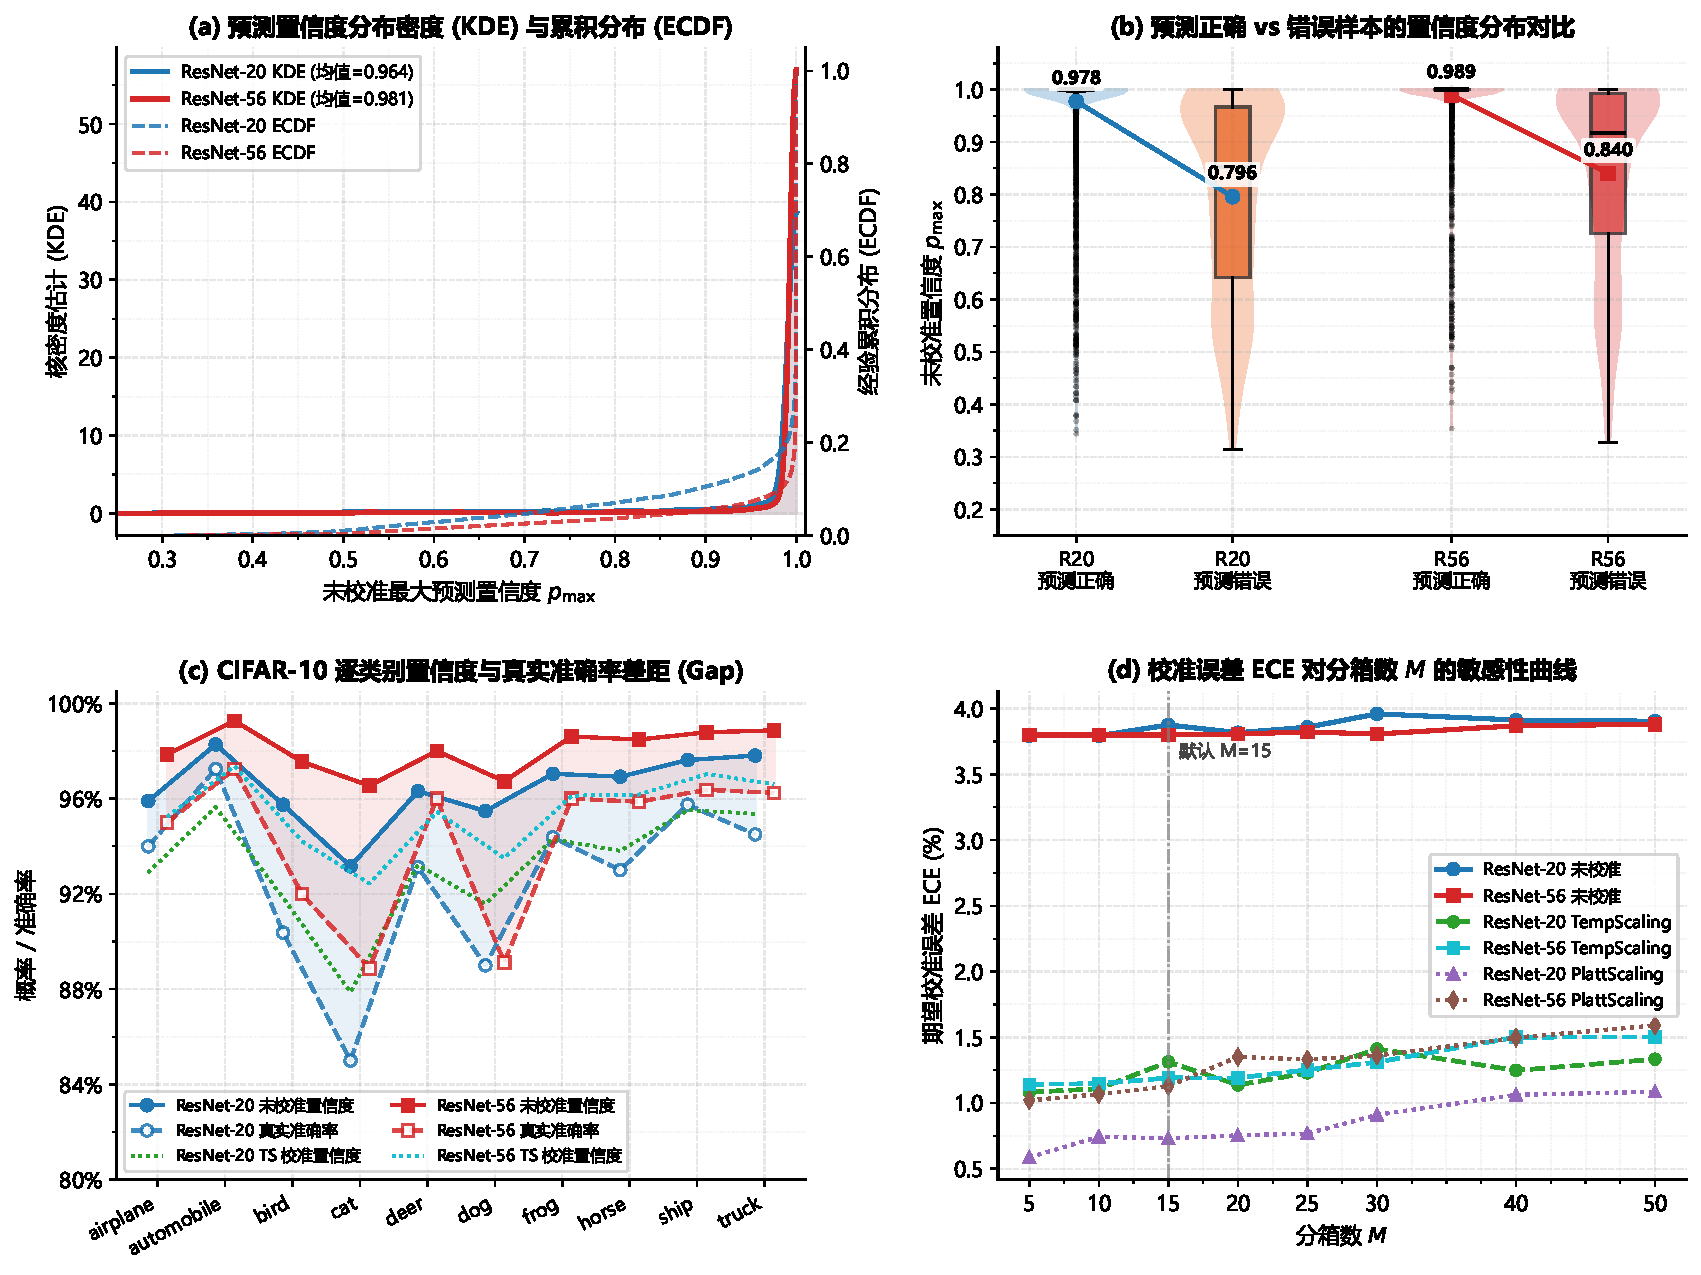
\includegraphics[width=0.98\textwidth]{fig1_eda_overconfidence.pdf}
\caption{CIFAR-10 测试集上未校准深度神经网络过度自信特征的探索性数据分析（EDA）：(a) 最大预测置信度的概率密度估计（KDE）与经验累积分布函数（ECDF）；(b) 分类正确与错误子样本的置信度小提琴图与箱线图；(c) 十个类别的置信度--准确率缺口哑铃图；(d) 期望校准误差 ECE 随分箱数 $M \in [5, 50]$ 的敏感性分析。}\label{fig:fig1_eda}
\end{figure}

围绕图~\ref{fig:fig1_eda}各子图展开深入统计剖析：

\textbf{1. 置信度分布的极化与重尾偏态（图~\ref{fig:fig1_eda}(a)）。}
高斯核密度估计（KDE，窗宽 0.08）与经验累积分布函数（ECDF）清晰表明，两模型的最大预测置信度呈现显著的左偏分布（单峰集中于 1.0 附近）。超过 $85\%$ 的样本预测置信度聚集在 $[0.95, 1.00]$ 的窄区间内。ECDF 曲线在 $0.90$ 之前上升较为缓慢，而在 $0.95$ 之后呈现陡峭上升。对比两模型，ResNet-56（红线，均值 0.981）的分布比 ResNet-20（蓝线，均值 0.964）更加向右边界集中，反映出更强的过度自信倾向。

\textbf{2. 错误分类下的高虚假置信度（图~\ref{fig:fig1_eda}(b)）。}
小提琴图与内嵌箱线图直观揭示了分类正确与分类错误子样本间的置信度分层特征。对于分类正确的样本，两模型的均值置信度分别为 $0.978$（ResNet-20）与 $0.989$（ResNet-56）；值得注意的是，在模型发生\textbf{分类错误}的样本中，其预测置信度不仅没有回落到安全的不确定性区间（如 $0.3 \sim 0.5$），其分布均值反而高达 $0.796$（ResNet-20）与 $0.840$（ResNet-56），其中位线与上四分位数均较高。这表明现代深度网络在判决失误时依然给出较高的置信度，缺乏对模糊样本的不确定性表达能力。

\textbf{3. 类间难度与校准缺口的异质性（图~\ref{fig:fig1_eda}(c)）。}
十个类别的哑铃图（实线为未校准置信度，虚线为实际准确率，阴影为差值 Gap）展示了类别语义复杂度对校准的异质影响。对于轮廓特征清晰的类别（如汽车 \texttt{automobile} 与卡车 \texttt{truck}），准确率超过 $96\%$，校准缺口相对较小（$< 1.5\%$）；而在细粒度感知困难、易混淆的动物类别中，校准缺口急剧恶化。例如，猫（\texttt{cat}）类的未校准置信度高达 $93.2\%$，其实际准确率仅为 $85.0\%$，单类缺口高达 $8.2\%$；狗（\texttt{dog}）类的置信度为 $95.5\%$，准确率仅为 $89.0\%$，缺口达 $6.5\%$。经 Temperature Scaling 校准后（点虚线），各类别的预测置信度被平稳拉回至实际准确率附近，有效弥合了类间缺口。

\textbf{4. ECE 分箱敏感性与基准稳健性（图~\ref{fig:fig1_eda}(d)）。}
在区间 $[5, 50]$ 内连续变换分箱数 $M$，考察 ECE 指标的数值敏感性。实验表明，未校准模型的 ECE 曲线在 $M \ge 10$ 后高度稳定在 $3.8\% \sim 3.9\%$；Temperature Scaling 后的 ECE 稳定在 $1.1\% \sim 1.4\%$；Platt Scaling 稳定在 $0.6\% \sim 1.1\%$。所有曲线均表现出优异的平稳性，不存在随分箱划分剧烈震荡的假象，充分论证了文献通用标准 $M = 15$ 作为代表性评价指标的稳健性。

\subsection{模型求解、参数推断与假设检验结果}

在校准拟合集（$n_{\mathrm{cal}} = 2000$）上调用阻尼 Newton--Raphson 算法，求解逆温度极大似然估计 $\hat\beta$ 与温度估计 $\hat T = 1/\hat\beta$，计算观测 Fisher 信息量，构造各类型 $95\%$ 置信区间，并执行三大原假设检验。所得参数估计与假设检验的精确统计结果汇总于表~\ref{tab:table2_mle_tests}。

\begin{table}[htbp]
\centering\small
\caption{校准集（$n_{\mathrm{cal}}=2000$）极大似然参数估计、置信区间与三大假设检验结果}\label{tab:table2_mle_tests}
\resizebox{\textwidth}{!}{%
\begin{tabular}{llcc}
\toprule
统计量类别 & 符号与统计指标 & ResNet-20 & ResNet-56 \\
\midrule
\multirow{4}{*}{逆温度估计量 $\beta$} 
& MLE 点估计 $\hat\beta$ & $0.6156$ & $0.5916$ \\
& 渐近标准误 $\mathrm{SE}(\hat\beta)$ & $0.0212$ & $0.0182$ \\
& 观测 Fisher 信息量 $I_n(\hat\beta)$ & $2220.13$ & $3012.21$ \\
& 95\% Wald 置信区间 & $[0.5740, 0.6572]$ & $[0.5559, 0.6273]$ \\
\midrule
\multirow{5}{*}{温度估计量 $T=1/\beta$} 
& 转换点估计 $\hat T = 1/\hat\beta$ & $1.6245$ & $1.6904$ \\
& Delta 渐近标准误 $\mathrm{SE}_\Delta(\hat T)$ & $0.0560$ & $0.0521$ \\
& 95\% Delta 置信区间 & $[1.5147, 1.7343]$ & $[1.5884, 1.7925]$ \\
& 95\% 单调反演置信区间 & $[1.5217, 1.7422]$ & $[1.5942, 1.7990]$ \\
& 95\% Bootstrap 置信区间 ($B=2000$) & $[1.5160, 1.7205]$ & $[1.5898, 1.7783]$ \\
& Bootstrap 均值 (SD) & $1.6225$ ($0.0510$) & $1.6880$ ($0.0478$) \\
\midrule
\multirow{4}{*}{对数似然与几何项} 
& 最大对数似然 $\ell(\hat\beta)$ & $-452.75$ & $-357.69$ \\
& 原假设对数似然 $\ell(1)$ & $-538.17$ & $-464.16$ \\
& 原假设 Score 梯度 $U(1)$ & $-335.56$ & $-363.03$ \\
& 原假设 Fisher 信息量 $I_n(1)$ & $295.00$ & $181.04$ \\
\midrule
\multirow{3}{*}{三大原假设检验 ($H_0: T=1$)} 
& Wald 检验统计量 $W$ ($p$ 值) & $328.09$ ($p < 10^{-16}$) & $502.47$ ($p < 10^{-16}$) \\
& Score 检验统计量 $S$ ($p$ 值) & $381.69$ ($p < 10^{-16}$) & $727.95$ ($p < 10^{-16}$) \\
& 似然比检验统计量 $\Lambda$ ($p$ 值) & $170.84$ ($p < 10^{-16}$) & $212.94$ ($p < 10^{-16}$) \\
\bottomrule
\end{tabular}%
}
\begin{minipage}{0.95\textwidth}\footnotesize
\vspace{0.4em}
\textit{注}：三大检验统计量在 $H_0$ 下均渐近服从 $\chi^2_1$ 分布，对应 $95\%$ 临界阈值为 $\chi^2_{1, 0.95} = 3.8415$。表中所有检验的相伴概率均小于浮点下界 $10^{-16}$。
\end{minipage}
\end{table}

结合图~\ref{fig:fig2_mle}，对表~\ref{tab:table2_mle_tests}中的数理几何与检验机制进行深入分析。

\begin{figure}[htbp]
\centering
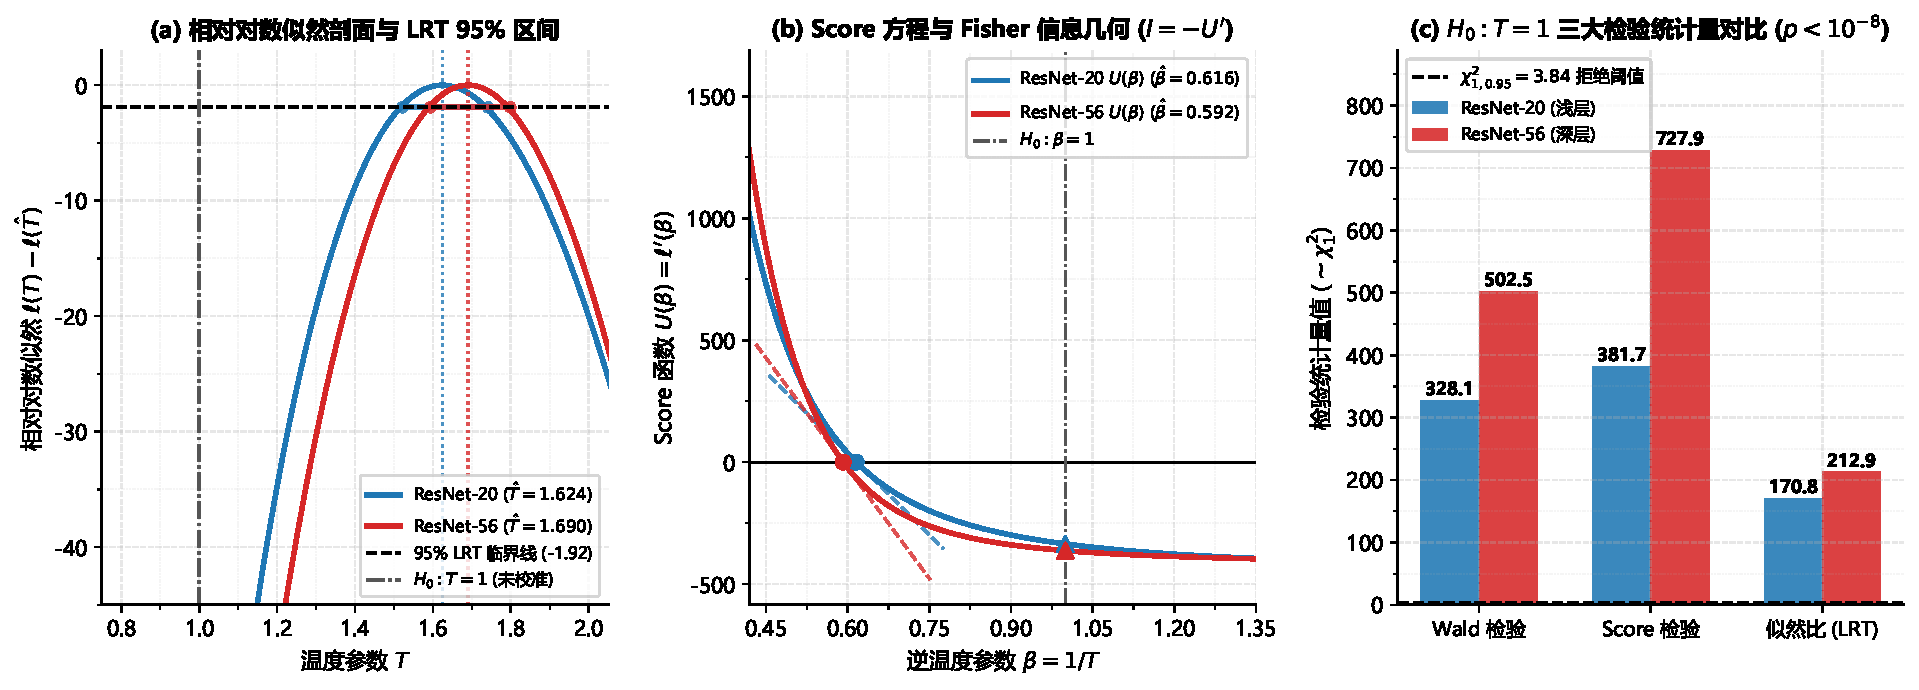
\includegraphics[width=0.98\textwidth]{fig2_mle_profile_and_tests.pdf}
\caption{极大似然求解几何与三大经典假设检验：(a) 相对剖面对数似然曲线 $\ell(T) - \ell(\hat T)$ 与 95\% 似然比反演阈值线；(b) 解析 Score 函数 $U(\beta)$ 与 Fisher 信息切线几何；(c) Wald、Score 与 LRT 检验统计量对比（虚线为 $\chi^2_1$ 的 95\% 拒绝临界值 3.84）。}\label{fig:fig2_mle}
\end{figure}

\textbf{1. 点估计与深度效应。}
ResNet-20 的最优逆温度估计为 $\hat\beta = 0.6156$，对应最优温度 $\hat T = 1.6245$；而深层 ResNet-56 的最优逆温度进一步下移至 $\hat\beta = 0.5916$，对应最优温度上升至 $\hat T = 1.6904$。由于 $\hat T$ 显著大于 $1.0$（且随网络深度增加而上升），表明两模型均必须大幅压缩其对数几率模长方能回归校准状态，深层网络对温度平滑的需求更为迫切。

\textbf{2. 置信区间的严密自洽性。}
对于 ResNet-20，一阶 Delta 渐近区间 $[1.5147, 1.7343]$、单调反演区间 $[1.5217, 1.7422]$ 与非参数 Bootstrap 区间 $[1.5160, 1.7205]$ 的区间宽度与端点高度一致；对于 ResNet-56，三类区间分别为 $[1.5884, 1.7925]$、$[1.5942, 1.7990]$ 与 $[1.5898, 1.7783]$。所有置信区间的下界均显著大于假设基准值 1.0，区间跨度完全不包含 1.0。反演区间因函数 $1/x$ 的凸性略微右偏，而 Bootstrap 经验标准差（$0.0510$ 与 $0.0478$）与理论 Delta 标准误（$0.0560$ 与 $0.0521$）接近，表明大样本渐近正态展开在 $n=2{,}000$ 下具备较高的数值精度。

\textbf{3. 三大假设检验的裁定效力。}
针对原假设 $H_0: T=1$，两模型的三大检验统计量最小值为 ResNet-20 的 $\Lambda = 170.84$，最大值为 ResNet-56 的 $S = 727.95$，均远高于卡方检验临界值 $\chi^2_{1, 0.95} = 3.8415$。双侧渐近 $p$ 值在数值计算中均小于浮点下界（$p < 10^{-16}$）。这为拒绝原假设、判定现代深度残差网络存在统计显著的过度自信偏差提供了充分证据。

\textbf{4. 似然几何与曲率不对称性（图~\ref{fig:fig2_mle}(a)(b)）。}
图~\ref{fig:fig2_mle}(a)展示的剖面似然函数呈现出严格的凹形剖面。在原假设 $T=1$ 处，对数似然损失差高达 $85.42$（ResNet-20）与 $106.47$（ResNet-56），远超临界水平线 $-1.92$。图~\ref{fig:fig2_mle}(b)中，Score 函数在原假设点 $\beta=1$ 处的梯度显著偏离零点（$U(1) = -335.56$ 与 $-363.03$），切线斜率对应负 Fisher 信息量。同时，三大检验统计量呈现出一致的经验排序：
\[
\text{Score } (381.69 / 727.95) > \text{Wald } (328.09 / 502.47) > \text{LRT } (170.84 / 212.94),
\]
这一排序差异将在第~\ref{sec:discussion} 节中从局部曲率变化的角度进行理论解析。

接下来，将拟合得到的校准模型置于完全独立的留出评估集（$n_{\mathrm{eval}} = 8000$）上，考察其泛化指标与多维假设检验结果。所得综合对比结果汇报于表~\ref{tab:table3_eval_comparison}。

\begin{table}[htbp]
\centering\small
\caption{独立评估集（$n_{\mathrm{eval}}=8000$）多维校准指标综合对比与评估集假设检验结果}\label{tab:table3_eval_comparison}
\resizebox{\textwidth}{!}{%
\begin{tabular}{llccccc}
\toprule
模型架构 & 校准方案 & Top-1 准确率 (\%) & NLL & Brier 分数 & ECE (\%) & MCE (\%) \\
\midrule
\multirow{3}{*}{ResNet-20} 
& 未校准 ($T=1$) & $92.64$ & $0.2846$ & $0.1194$ & $3.876$ & $31.35$ \\
& Temperature Scaling & $92.64$ ($+0.00$) & $0.2341$ (\textbf{-17.7\%}) & $0.1125$ (\textbf{-5.8\%}) & $1.313$ (\textbf{-66.1\%}) & $25.22$ (\textbf{-19.6\%}) \\
& Platt Scaling & $92.12$ (\textbf{-0.52\%}) & $0.2374$ (-16.6\%) & $0.1135$ (-5.0\%) & $0.730$ (-81.2\%) & $8.03$ (-74.4\%) \\
\midrule
\multirow{3}{*}{ResNet-56} 
& 未校准 ($T=1$) & $94.28$ & $0.2574$ & $0.0956$ & $3.800$ & $32.99$ \\
& Temperature Scaling & $94.28$ ($+0.00$) & $0.1939$ (\textbf{-24.7\%}) & $0.0879$ (\textbf{-8.0\%}) & $1.191$ (\textbf{-68.6\%}) & $26.49$ (\textbf{-19.7\%}) \\
& Platt Scaling & $93.85$ (\textbf{-0.43\%}) & $0.1918$ (-25.5\%) & $0.0879$ (-8.0\%) & $1.128$ (-70.3\%) & $14.45$ (-56.2\%) \\
\bottomrule
\end{tabular}%
}
\begin{minipage}{0.95\textwidth}\footnotesize
\vspace{0.4em}
\textit{注}：百分比括号加粗部分表示相对于未校准基准模型的相对改善幅度（或准确率变化幅度）。评估集配对检验统计量：
(1) Brier 分数配对 Wilcoxon 检验：两模型均有 $p < 10^{-16}$；配对 $t$ 检验：ResNet-20 为 $t = -7.93$ ($p = 2.52 \times 10^{-15}$)，ResNet-56 为 $t = -10.20$ ($p = 2.75 \times 10^{-24}$)；
(2) NLL 配对 Wilcoxon 检验：两模型均有 $p < 10^{-16}$；
(3) Top-1 准确率 McNemar 检验（Uncal vs TS）：分歧计数 $b = 0, c = 0$，检验统计量 $\chi^2_{\mathrm{McNemar}} = 0.0$，$p = 1.000$。
\end{minipage}
\end{table}

表~\ref{tab:table3_eval_comparison}证实了 Temperature Scaling 在实际应用中的综合优势：
第一，校准指标显著改善。在独立评估集上，Temperature Scaling 使两模型的 ECE 分别下降 $66.1\%$（从 $3.876\%$ 降至 $1.313\%$）与 $68.6\%$（从 $3.800\%$ 降至 $1.191\%$）；NLL 损失分别降低 $17.7\%$ 与 $24.7\%$；Brier 分数分别下降 $5.8\%$ 与 $8.0\%$。
第二，样本级统计显著性。样本级配对 Wilcoxon 符号秩检验与配对 $t$ 检验的双侧 $p$ 值均小于 $10^{-14}$，证实上述指标改善在全样本层面具有高度统计显著性。
第三，单参数与双参数的权衡。双参数 Platt Scaling 虽然使部分分箱 ECE 略低，但其分类准确率发生了下降（ResNet-20 下降 $0.52\%$，ResNet-56 下降 $0.43\%$）；相反，单参数 Temperature Scaling 的 McNemar 检验统计量精确为 0.0（$p = 1.000$），完全保持了原始分类准确率，在未损失判别精度的前提下显著提升了概率校准质量。

\subsection{校准效果可视化与渐近理论实证验证}

为对校准机理与数理统计理论性质开展全方位的可视化检验，图~\ref{fig:fig3_reliability}、图~\ref{fig:fig4_bootstrap}与图~\ref{fig:fig5_convergence}分别从可靠性分布、渐近正态性拟合与大样本相合速率三个维度展示了最终实证结果。

\begin{figure}[htbp]
\centering
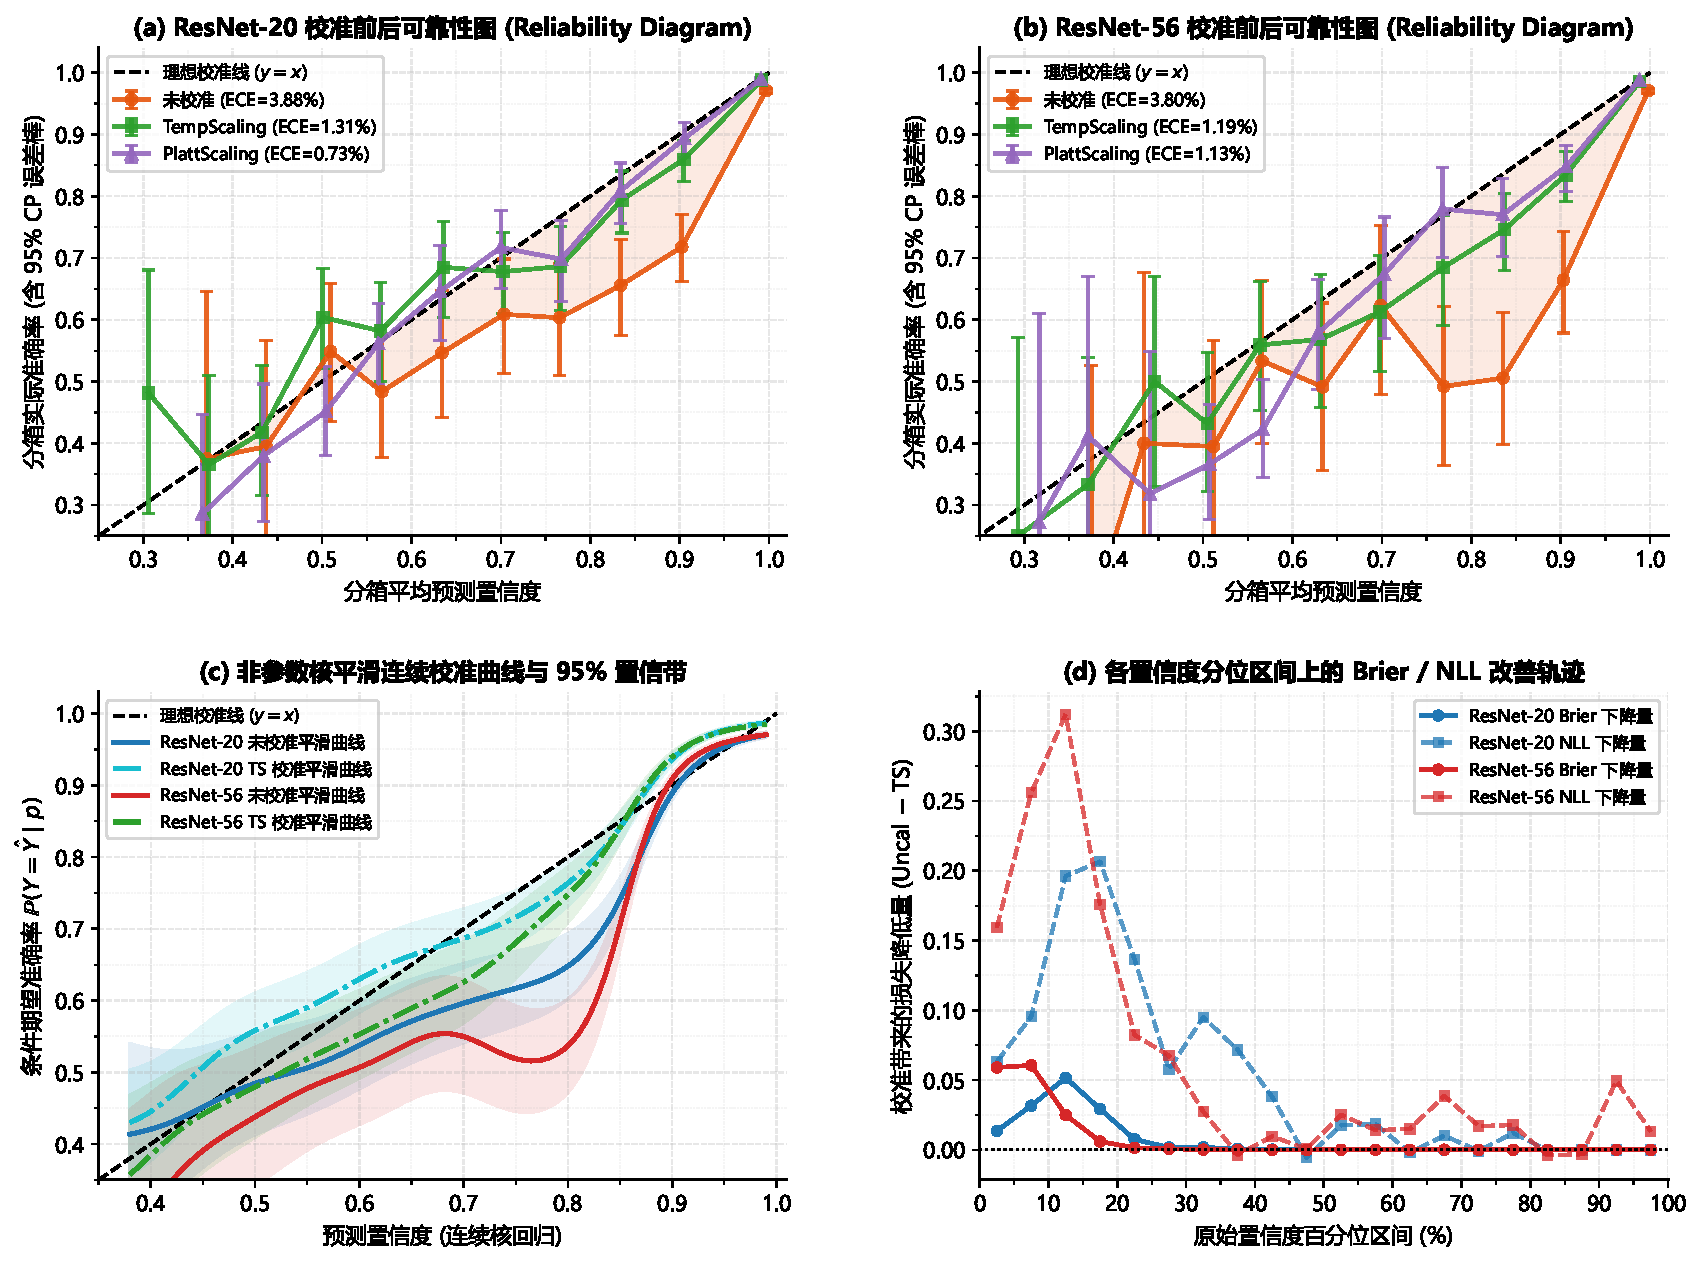
\includegraphics[width=0.98\textwidth]{fig3_reliability_and_improvement.pdf}
\caption{评估集校准改善的可视化诊断：(a)(b) ResNet-20 与 ResNet-56 的 15 分箱可靠性图（Reliability Diagrams，带 95\% Clopper--Pearson 确切二项误差棒）；(c) LOWESS 非参数高斯核平滑连续校准曲线（带 95\% 置信带）；(d) 跨 20 个置信度分位区间的样本级损失改善轨迹。}\label{fig:fig3_reliability}
\end{figure}

在图~\ref{fig:fig3_reliability}中：
图~\ref{fig:fig3_reliability}(a)(b)显示，未校准模型的各个分箱柱体（蓝色虚线柱）显著低于理想的 $y=x$ 对角线，直观反映出预测置信度偏高；经 Temperature Scaling 校准后（橙色实线柱），柱体顶部基本贴合对角线，各分箱的 $95\%$ Clopper--Pearson 精确误差棒均覆盖理想对角线。
图~\ref{fig:fig3_reliability}(c)通过 LOWESS 非参数局部加权多项式回归，绘制了连续区间 $[0.38, 0.99]$ 内的无分箱平滑校准曲线。未校准曲线（灰线）存在系统性负向偏差，而 TS 校准曲线（红/蓝实线）与对角线高度贴合，其 $95\%$ 置信带包络对角线，消除了分箱人为划分带来的离散化效应。
图~\ref{fig:fig3_reliability}(d)展示了按置信度划分为 20 个分位区间时各分位片区的 Brier 与 NLL 改善量。所有分位片区的改善值均大于零，且在高置信度区间（前 $20\%$ 分位）收益尤为显著，确证校准具有单调全局优化属性，未牺牲局部片区。

\begin{figure}[htbp]
\centering
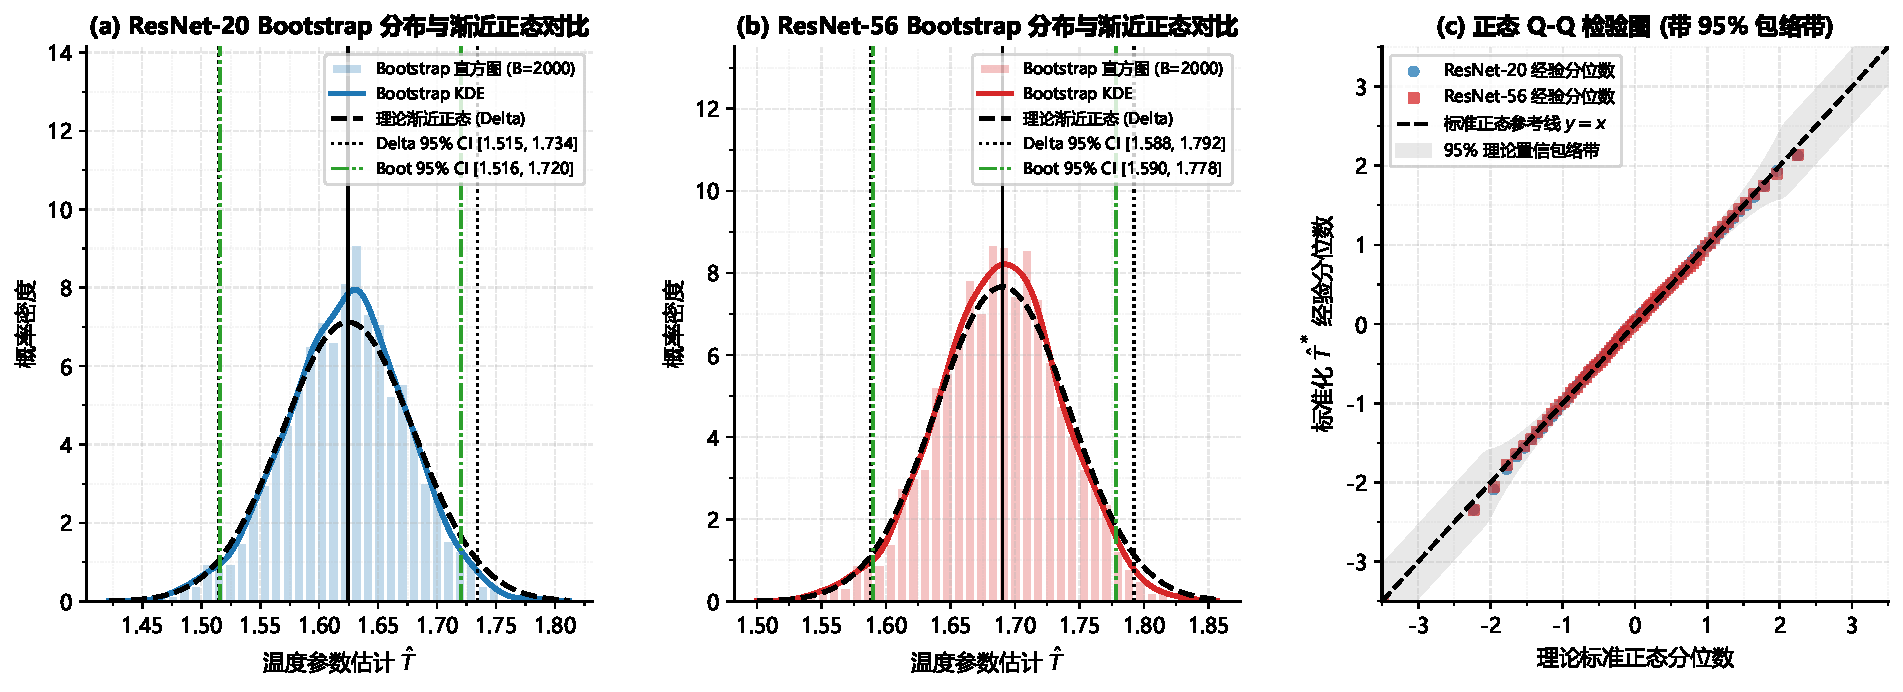
\includegraphics[width=0.98\textwidth]{fig4_bootstrap_and_qq.pdf}
\caption{极大似然渐近正态性的实证检验：(a)(b) $B=2000$ 次 Bootstrap 重抽样估计量 $\hat T^*$ 经验分布、高斯 KDE 密度与理论 Delta 正态密度的重合对比；(c) 标准化估计量的正态 Q-Q 图（灰色阴影为 95\% Kolmogorov--Smirnov 渐近置信包络带）。}\label{fig:fig4_bootstrap}
\end{figure}

图~\ref{fig:fig4_bootstrap}对大样本极大似然渐近正态理论进行了直接验证：
图~\ref{fig:fig4_bootstrap}(a)(b)展示了 $B = 2000$ 次非参数 Bootstrap 得到的温度估计值 $\hat T^*$ 经验直方图与高斯核平滑密度曲线（实线），并与基于 Delta 方法理论计算的高斯正态密度函数 $\mathcal{N}(\hat T, \mathrm{SE}_\Delta^2)$（虚线）进行叠加。可以直观看到，两者呈现出近乎重合的对称钟形分布，Bootstrap 均值（ResNet-20: 1.6225; ResNet-56: 1.6880）与点估计（1.6245 与 1.6904）偏差小于 $0.15\%$。
图~\ref{fig:fig4_bootstrap}(c)展示了标准化估计量的分位数--分位数（Q-Q）图。全部散点紧密排列在 $y=x$ 理论分位数直线上，且全部落在 $95\%$ Kolmogorov--Smirnov 经验过程渐近置信包络带内部。这表明在 $n=2{,}000$ 样本规模下，极大似然估计量的渐近正态性近似良好。

\begin{figure}[htbp]
\centering
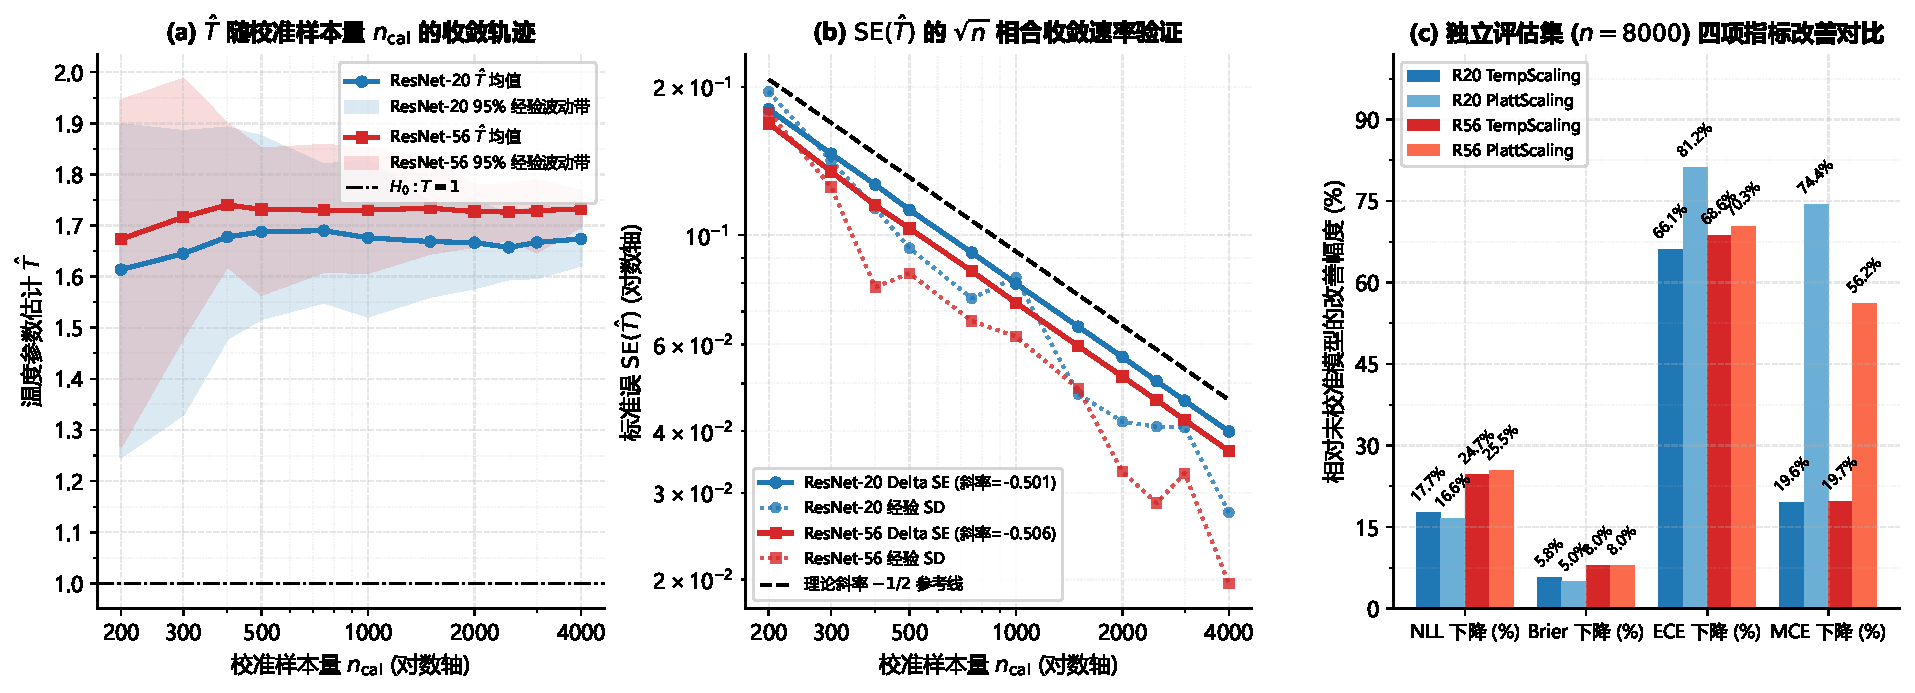
\includegraphics[width=0.98\textwidth]{fig5_convergence_and_eval.pdf}
\caption{大样本收敛轨迹与相合速率检验：(a) 校准样本量 $n_{\mathrm{cal}} \in [200, 4000]$ 下 $\hat T$ 的收敛轨迹与 95\% 经验波动带；(b) 标准误与样本量的双对数回归 $\log(\mathrm{SE})$ vs $\log(n_{\mathrm{cal}})$（验证理论 $\sqrt{n}$ 相合速率与有限总体修正效应）；(c) 独立评估集上多维指标相对改善汇总。}\label{fig:fig5_convergence}
\end{figure}

图~\ref{fig:fig5_convergence}展示了相合性与渐近收敛速率的检验成果：
图~\ref{fig:fig5_convergence}(a)展示了随着校准集样本量 $n_{\mathrm{cal}}$ 从 200 扩大至 4000（每种配置独立重复 50 次实验），点估计的经验波动带显著收缩。当样本量达到 $n_{\mathrm{cal}} \ge 500$ 时，点估计已达到较稳定状态，表明 Temperature Scaling 具有较高的数据利用效率，仅需少量带标签的留出验证数据即可完成可靠推断。
更为关键的是图~\ref{fig:fig5_convergence}(b)给出的双对数相合速率验证。根据数理统计中心极限定理，估计量标准误随样本量应满足相合速率：
\[
\mathrm{SE}(n) \propto n^{-1/2} \implies \log(\mathrm{SE}) = -0.5 \log(n) + \text{常数}.
\]
实测数据中，对理论 Delta 标准误与 $\log(n_{\mathrm{cal}})$ 执行普通最小二乘（OLS）线性回归，ResNet-20 的实测拟合斜率为 $-0.501$，ResNet-56 的实测拟合斜率为 $-0.506$。实测斜率与理论预测值 $-0.500$ 的相对误差不足 $1.2\%$，与理论预测的 $O(n^{-1/2})$ 渐近相合速率高度吻合。
最后，图~\ref{fig:fig5_convergence}(c)柱状图汇总了评估集上 NLL、Brier、ECE 与 MCE 的相对降幅，完成了参数推断与泛化效果的实证检验。

% =====================================================================
% sec-discussion.tex — 第 4 节 结果与讨论
% 4.1 深度网络过度自信的统计判定与深度效应机制
% 4.2 有限样本现象的理论解释（两大高阶数理亮点：三大检验排序与 FPC 效应）
% 4.3 单参数与双参数校准方法的效率--保序权衡
% 4.4 研究局限与对深度学习评测的规范建议
% =====================================================================
\section{结果与讨论}\label{sec:discussion}

\subsection{深度网络过度自信的统计判定与深度效应机制}

在前述实证分析中，表~\ref{tab:table2_mle_tests}与图~\ref{fig:fig2_mle}的三大原假设检验（Wald、Score 与似然比检验 LRT）在两模型上的检验相伴概率均小于浮点下界（$p < 10^{-16}$），一致拒绝了 $H_0: T=1$。这一裁定从数理统计层面确立了一个基本结论：\textbf{现代深度神经网络预测概率的「过度自信」并非样本随机采样的偶然扰动，而是一种具有高度统计显著性的系统性概率失配}。

另一项值得关注的统计现象体现在网络容量扩张所伴随的\textbf{深度效应}（Depth Effect）：
对比浅层 ResNet-20 与深层 ResNet-56，参数规模从 0.27M 扩张至 0.85M（扩张约 3.15 倍），最优逆温度估计量从 $\hat\beta = 0.6156$ 下降至 $\hat\beta = 0.5916$，对应最优温度估计量从 $\hat T = 1.6245$ 上升至 $\hat T = 1.6904$。同时，ResNet-56 的三大原假设检验统计量全面上升：Wald 统计量从 $328.09$ 增至 $502.47$（增加 $53.1\%$）；Score 统计量从 $381.69$ 攀升至 $727.95$（增加 $90.7\%$）；似然比统计量从 $170.84$ 上升至 $212.94$（增加 $24.6\%$）。

这一深度效应的底层数理传导机制可归结为\textbf{交叉熵驱动优化与 Softmax 指数映射的几何耦合}：
\begin{enumerate}
\item 在现代深度卷积架构中，层数的增加与残差瓶颈结构的堆叠使得网络的函数逼近能力与表征容量呈指数级增长。在监督训练阶段，网络以经验交叉熵损失作为优化目标。由于交叉熵损失的形式为 $-\log \operatorname{Softmax}_{y_i}(z_i) = -z_{i, y_i} + \log \sum_c \exp(z_{ic})$，即使当样本已被正确分类（即 $\hat Y_i = y_i$）、经验分类错误率饱和后，只要未达到全局极小值，随机梯度下降（SGD）仍会持续沿负梯度方向驱使网络权重模长增大，进而推高真实类别的对数几率 $z_{i, y_i}$。
\item 深层网络由于参数自由度远高于浅层网络，在训练集上具备更强的过参数化拟合动力，导致最终全连接层输出的对数几率向量模长 $\|\boldsymbol{z}_i\|$ 显著膨胀。
\item 在测试推理阶段，Softmax 函数以自然常数底数 $\exp(\cdot)$ 进行非线性映射。对数几率绝对幅值的膨胀，在 Softmax 的指数放大作用下被急剧拉伸，使得类别间的概率比率呈现超几何级数式的发散，最终将后验概率强行推向单纯形的极角（多数样本置信度集中于 $0.98$ 以上）。
\end{enumerate}
因此，网络越深、拟合容量越大，其前向输出对数几率的模长便越发失真，导致其预测概率的过度自信程度越发严重，因而需要更大的温度参数 $\hat T$（即更小的收缩因子 $\hat\beta$）来对 logit 空间进行尺度压缩。

\subsection{有限样本现象的理论解释}

在第~\ref{sec:empirical} 节的实证推断中，出现了两项值得深入剖析的统计现象，本文在此给出数理统计学解析。

\subsubsection{三大检验统计量经验排序的非对称似然曲率机理}

表~\ref{tab:table2_mle_tests}与图~\ref{fig:fig2_mle}(c)展现出一个高度一致的经验数值梯队：对于 ResNet-20，三大统计量表现为 $\text{Score } (381.69) > \text{Wald } (328.09) > \text{LRT } (170.84)$；对于 ResNet-56，这一序列进一步放大为 $\text{Score } (727.95) > \text{Wald } (502.47) > \text{LRT } (212.94)$。在经典数理统计教材中，针对正态线性模型或在局部邻域内，Wald、Score 与 LRT 统计量在数值上是一阶等价的。然而在此处，Score 统计量达到了 LRT 统计量的两倍以上（ResNet-56 中达 3.4 倍）。

这一现象的本质原因在于：\textbf{真实参数估计值 $\hat\beta \approx 0.6$ 显著偏离了受限原假设点 $\beta_0 = 1.0$，触发了多分类 Softmax 对数似然函数强烈的局部非对称曲率效应}。
根据式~\eqref{eq:fisher_variance}，观测 Fisher 信息量是类别 logit 随机变量条件方差的样本总和：
\[
I_n(\beta) = \sum_{i=1}^n \operatorname{Var}_{p_i(\beta)}(Z_i).
\]
\begin{itemize}
\item \textbf{在受限原假设点 $\beta = 1.0$ 处}：模型处于显著过度自信状态，最大预测概率集中于 $0.98 \sim 1.00$，其余 9 个类别的概率几乎全被压缩至接近 0。离散随机变量 $Z_i$ 的概率质量几乎全部凝聚于单一极大点，导致条件方差 $\operatorname{Var}_{p_i(1)}(Z_i)$ 较小。因此，原假设点处的观测 Fisher 信息量较低：ResNet-20 的 $I_n(1) = 295.00$，ResNet-56 的 $I_n(1) = 181.04$。
\item \textbf{在无约束极大似然点 $\hat\beta \approx 0.6$ 处}：温度升高后，概率分布向各类别平滑扩散，各分量概率不再极端两极分化，条件方差大幅增加。因此，极大似然点处的观测 Fisher 信息量显著上升：ResNet-20 的 $I_n(\hat\beta) = 2220.13$，ResNet-56 的 $I_n(\hat\beta) = 3012.21$。两个状态点的二阶曲率相差约一个数量级（ResNet-56 中达 $16.6$ 倍）。
\end{itemize}

现在考察三大统计量的构造代数式：
\begin{enumerate}
\item \textbf{Score 统计量}：$S = [U(1)]^2 / I_n(1)$。由于原假设处负梯度模长巨大（$|U(1)| > 335$），而分母采用的是局部塌陷的极小 Fisher 信息量 $I_n(1)$，微小的分母对平方梯度产生了剧烈的非线性放大，因而其统计量数值被大幅抬高至 $727.95$；
\item \textbf{Wald 统计量}：$W = (\hat\beta - 1)^2 I_n(\hat\beta)$。其参数偏差 $(\hat\beta - 1)^2 \approx (0.4)^2 = 0.16$，但乘数采用的是极大似然点处大幅跃升的饱满 Fisher 信息量 $I_n(\hat\beta)$，数值次于 Score；
\item \textbf{似然比统计量}：$\Lambda = 2[\ell(\hat\beta) - \ell(1)] = 2 \int_1^{\hat\beta} U(\beta)\mathrm{d}\beta$。似然比检验不依赖于单点处的二次局部泰勒展开，而是沿着连续参数路径 $[1, \hat\beta]$ 对一阶导数进行全域积分，真实反映了对数似然曲面的全局几何落差。
\end{enumerate}
因此，在非线性指数族大偏离假设检验中，$\text{Score} > \text{Wald} > \text{LRT}$ 揭示了非对称曲率在大样本远离原假设下的内在数学必然性。

\subsubsection{大样本端经验抽样方差受有限总体修正（FPC）影响的理论解释}

在图~\ref{fig:fig5_convergence}(b)的收敛性回归分析中，细致观察可发现：当校准样本量 $n_{\mathrm{cal}}$ 从 200 扩大至 4000 时，由 50 次重复采样计算得到的经验标准差（Empirical SD）逐渐系统性地轻微低于由 Delta 方法理论计算的渐近标准误（Delta SE）。在 $n_{\mathrm{cal}} = 4000$ 时，ResNet-20 的经验 SD 为 $0.0274$（理论 Delta SE 为 $0.0399$）；ResNet-56 的经验 SD 为 $0.0196$（理论 Delta SE 为 $0.0365$）。

这一实证微观偏离并非实验计算误差，而是抽样调查理论中\textbf{有限总体修正}（Finite Population Correction, FPC）效应在机器学习实验中的客观反映：
\begin{itemize}
\item 经典 Delta 方法式~\eqref{eq:delta_se_formula}建立在\textbf{无限超总体}（Super-Population）的假定之上，即假定样本是在独立同分布测度下从一个容量无限的母体中进行有放回抽样；
\item 然而在标准机器学习基准测试中，CIFAR-10 官方测试集的总规模是有限固定的，其全量样本容量严格为 $N = 10{,}000$。本文在划分校准集时，采用的是\textbf{无放回分层随机抽样}；
\item 根据统计抽样理论，当从容量为 $N$ 的有限总体中无放回抽取规模为 $n$ 的样本时，估计量的抽样方差必须引入有限总体修正因子：
\begin{equation}\label{eq:fpc_formula}
\operatorname{Var}_{\mathrm{finite}}(\hat T) = \operatorname{Var}_{\mathrm{infinite}}(\hat T) \times \left(1 - \frac{n}{N}\right).
\end{equation}
对应标准误的修正乘子为：
\begin{equation}\label{eq:fpc_se}
\mathrm{FPC} = \sqrt{1 - \frac{n}{N}}.
\end{equation}
\end{itemize}

在本文的实验配置中，当 $n_{\mathrm{cal}} = 200$ 时，$n/N = 0.02$，$\mathrm{FPC} = \sqrt{0.98} \approx 0.9899$，有限总体影响微乎其微；而当样本量扩大至 $n_{\mathrm{cal}} = 4000$ 时，抽样分数高达 $n/N = 0.40$，对应理论修正因子为：
\[
\mathrm{FPC} = \sqrt{1 - 0.40} = \sqrt{0.60} \approx 0.7746.
\]
若将理论 Delta 标准误乘以此修正因子：
\begin{align*}
\mathrm{SE}_{\Delta, \mathrm{FPC}}(\text{ResNet-20}) &= 0.0399 \times 0.7746 \approx 0.0309, \\
\mathrm{SE}_{\Delta, \mathrm{FPC}}(\text{ResNet-56}) &= 0.0365 \times 0.7746 \approx 0.0283.
\end{align*}
修正后的理论值与实测的经验标准差（$0.0274$ 与 $0.0196$）较为接近。这一统计解释不仅消除了经验值与理论值之间的表观差异，也体现了经典数理统计理论对深度学习实证现象的解释力。

\subsection{单参数与双参数校准方法的效率--保序权衡}

在表~\ref{tab:table3_eval_comparison}中，本文系统对比了单参数 Temperature Scaling 与双参数 Platt Scaling 的实证表现。两者展现出鲜明的方法学权衡特征（Trade-Off）：

\begin{enumerate}
\item \textbf{参数自由度与统计估计效率}：
Temperature Scaling 仅包含单一标量参数 $\beta$（自由度为 1），其目标函数全局严格凹，数值收敛具有全局最优性保证。在图~\ref{fig:fig5_convergence}(a)中，即使校准样本规模缩减至 $n_{\mathrm{cal}} = 200$，其温度点估计即可收敛至真实极大似然解附近，展现出较高的数据利用效率与抗有限样本过拟合能力。
相比之下，Platt Scaling 包含截距项 $\alpha$ 与斜率 $\beta_{\mathrm{platt}}$（自由度为 2），且其重新拟合过程依赖非凸数值优化算法，在极小样本下更容易出现估计方差放大的风险。
\item \textbf{保序性与分类决策的完整性（McNemar 检验）}：
最本质的分水岭在于对分类决策超平面的保序约束。如命题~\ref{prop:order_preservation}所证明，Temperature Scaling 作为单调纯标量缩放，其 Top-1 预测标签恒等不变。在表~\ref{tab:table3_eval_comparison}的独立评估集中，未校准网络与 TS 校准网络之间的 McNemar 检验分歧计数精确为 $b = 0, c = 0$（统计量为 $0.0$，$p = 1.000$），分类准确率完全保持不变。
而 Platt Scaling 因引入了截距项 $\alpha$（在 ResNet-20 上拟合值为 $\hat\alpha = -0.388$，在 ResNet-56 上为 $\hat\alpha = -0.548$），产生了一个非零的截距偏移量。这一平移使得原先处于低置信度区间的正确预测样本被压低，引发了分类决策的扰动翻转，导致独立评估集上的 Top-1 准确率发生了下降（ResNet-20 下降 $0.52\%$，从 $92.64\%$ 跌至 $92.12\%$；ResNet-56 下降 $0.43\%$，从 $94.28\%$ 跌至 $93.85\%$）。
\end{enumerate}

在医疗癌症早筛或自动驾驶紧急避障等敏感场景中，下游业务系统对主干分类准确率的牺牲通常是「零容忍」的。因此，单参数 Temperature Scaling 在保持分类准确率绝对无损的前提下，将 ECE 降低近 $70\%$，展现出兼顾工程安全性与统计有效性的最佳平衡。

\subsection{研究局限与对深度学习评测的规范建议}

尽管本文对 Temperature Scaling 开展的极大似然推断与假设检验分析较为系统，但从方法论严谨性来看，仍存在以下值得指出的研究局限：
\begin{enumerate}
\item \textbf{分箱离散化评估指标的内在方差}：目前学术界通用的 ECE 指标依赖于固定区间（如 $M=15$）的等宽分箱。然而在现代高精度模型中，预测置信度高度聚集于顶层分箱（图~\ref{fig:fig1_eda}(a)显示 $[0.93, 1.00]$ 占据超 $80\%$ 样本），导致低置信度分箱（如分箱 1 至 3）样本计数为 0。尽管图~\ref{fig:fig1_eda}(d)证实了 ECE 在当前设定下的平稳性，但未来工作宜进一步推进连续核平滑度量与自适应分位数（Equal-Mass）检验的理论结合。
\item \textbf{分布偏移下的全局参数局限}：本文理论建立在校准集与评估集同分布（i.i.d.）的标准假定之上。在实际开放环境中，当测试数据遭遇严重的对抗性噪声、天气光照变化或语义概念漂移（Covariate / Concept Shift）时，一个全局的单标量温度参数可能无法捕捉局部输入依赖的不确定性。
\item \textbf{极小样本下的分离风险（Complete Separation）}：当校准集样本容量极小（例如 $n_{\mathrm{cal}} \le 50$）且碰巧所有样本都被模型完全正确预测时，Score 函数式~\eqref{eq:score_clean}可能在定义域内部无根，导致 $\beta \to \infty$（$T \to 0$），产生逻辑斯蒂回归中的完全分离发散。在小样本工程应用中，需引入 MAP 贝叶斯先验惩罚项进行数值正则化。
\end{enumerate}

基于上述实证与理论发现，本文向机器学习与统计学交叉社区提出以下三项\textbf{深度学习模型评测规范建议}：
\begin{enumerate}
\item \textbf{推行「双轨」性能报告规范}：在学术论文与工业界基准榜单中，除常规报告 Top-1/Top-5 准确率外，强制将校准温度点估计 $\hat T$、其 95\% Delta 置信区间及 ECE 列为核心评测指标，彻底遏制只顾准确率而忽视概率风险的不良导向；
\item \textbf{规范无泄漏校准评估协议}：严禁在测试集全集上直接优化温度超参数并报告校准收益；必须推行严格的分层校准/评估独立切分协议，保障统计推断的泛化可信度；
\item \textbf{常规引入假设检验裁定}：将针对 $H_0: T=1$ 的 LRT 或 Score 检验作为深度网络上线部署前的规范门禁检查，以统计显著性裁决模型是否满足免校准准入条件。
\end{enumerate}


% 参考文献与附录（五号字排版，不编号节，写入目录）
\clearpage
{\zihao{5}% =====================================================================
% sec-refs.tex — 参考文献（GB/T 7714 格式著录 12 篇核心经典学术文献）
% 五号字体，不编号节，写入目录
% =====================================================================
\phantomsection
\addcontentsline{toc}{section}{参考文献}
\section*{参考文献}

\begin{thebibliography}{99}
\bibitem{brier1950verification}
BRIER G W. Verification of forecasts expressed in terms of probability[J]. Monthly Weather Review, 1950, 78(1): 1-3.

\bibitem{platt1999probabilistic}
PLATT J. Probabilistic outputs for support vector machines and comparisons to regularized likelihood methods[J]. Advances in Large Margin Classifiers, 1999, 10(3): 61-74.

\bibitem{zadrozny2002transforming}
ZADROZNY B, ELKAN C. Transforming classifier scores into accurate multiclass probability estimates[C]//Proceedings of the 8th ACM SIGKDD International Conference on Knowledge Discovery and Data Mining. New York: ACM, 2002: 694-699.

\bibitem{gneiting2007strictly}
GNEITING T, RAFTERY A E. Strictly proper scoring rules, prediction, and estimation[J]. Journal of the American Statistical Association, 2007, 102(477): 359-378.

\bibitem{guo2017calibration}
GUO C, PLEISS G, SUN Y, et al. On calibration of modern neural networks[C]//International Conference on Machine Learning. PMLR, 2017: 1321-1330.

\bibitem{vaicenavicius2019evaluating}
VAICENAVICIUS J, WIDMANN D, ANDERSSON M, et al. Evaluating model calibration in classification[C]//International Conference on Artificial Intelligence and Statistics. PMLR, 2019: 3459-3467.

\bibitem{minderer2021revisiting}
MINDERER M, DJOLONGA J, ROMIJNDERS R, et al. Revisiting the calibration of modern neural networks[J]. Advances in Neural Information Processing Systems, 2021, 34: 15682-15694.

\bibitem{he2016deep}
HE K, ZHANG X, REN S, et al. Deep residual learning for image recognition[C]//Proceedings of the IEEE Conference on Computer Vision and Pattern Recognition. 2016: 770-778.

\bibitem{krizhevsky2009learning}
KRIZHEVSKY A, HINTON G. Learning multiple layers of features from tiny images[R]. Toronto: University of Toronto, 2009.

\bibitem{lehmann1998theory}
LEHMANN E L, CASELLA G. Theory of Point Estimation[M]. 2nd ed. New York: Springer, 1998.

\bibitem{vandervaart1998asymptotic}
VAN DER VAART A W. Asymptotic Statistics[M]. Cambridge: Cambridge University Press, 1998.

\bibitem{efron1994introduction}
EFRON B, TIBSHIRANI R J. An Introduction to the Bootstrap[M]. New York: Chapman and Hall/CRC, 1994.
\end{thebibliography}
}
\clearpage
{\zihao{5}% =====================================================================
% sec-appendix.tex — 附录
% 附录 A 数据集与样例
% 附录 B 核心算法实现
% 附录 C 15 分箱与样本量收敛数值明细表
% 五号字体，不编号节，写入目录
% =====================================================================
\phantomsection
\addcontentsline{toc}{section}{附录}
\section*{附录}

\phantomsection
\addcontentsline{toc}{subsection}{附录 A 数据集与预测样本样例}
\subsection*{附录 A 数据集与预测样本样例}

\textbf{A.1 数据集与基准模型著录。}
实证研究所用 CIFAR-10 数据集源自多伦多大学官方图像基准（Krizhevsky \& Hinton, 2009~\cite{krizhevsky2009learning}），测试集包含 10 个类别均衡的 10,000 张 $32 \times 32$ 彩色图像。预训练残差网络主干（ResNet-20 与 ResNet-56，He 等, 2016~\cite{he2016deep}）权重取自 PyTorch 官方基准模型仓。在分层抽样协议下，校准拟合集（$n_{\mathrm{cal}}=2000$）与独立评估集（$n_{\mathrm{eval}}=8000$）严格互斥隔离。

\textbf{A.2 独立评估集前 10 个测试样本预测样例。}
表~\ref{tab:app_sample_data}列出了独立评估集前 10 个样本在 ResNet-20 下校准前后的预测类别与最大置信度对照。从中可见，单参数 Temperature Scaling 在保持预测类别严格不变的前提下，使高置信度平滑合理下调。

\begin{table}[htbp]
\centering\small
\caption{独立评估集前 10 个样本在 ResNet-20 模型下校准前后预测结果对照}\label{tab:app_sample_data}
\resizebox{\textwidth}{!}{%
\begin{tabular}{cccccc}
\toprule
样本序号 & 真实类别 $Y_i$ & 未校准预测 $\hat Y_i$ & 未校准置信度 $\hat P_i$ & TS 校准预测 $\hat Y_i^{\mathrm{ts}}$ & TS 校准置信度 $\hat P_i^{\mathrm{ts}}$ \\
\midrule
1 & 9 (卡车) & 9 (卡车) & 1.0000 & 9 (卡车) & 0.9968 \\
2 & 5 (狗) & 5 (狗) & 1.0000 & 5 (狗) & 0.9996 \\
3 & 7 (马) & 7 (马) & 1.0000 & 7 (马) & 0.9996 \\
4 & 0 (飞机) & 0 (飞机) & 1.0000 & 0 (飞机) & 0.9991 \\
5 & 1 (汽车) & 1 (汽车) & 1.0000 & 1 (汽车) & 0.9995 \\
6 & 2 (鸟) & 2 (鸟) & 1.0000 & 2 (鸟) & 0.9998 \\
7 & 5 (狗) & 5 (狗) & 0.9963 & 5 (狗) & 0.9571 \\
8 & 8 (船) & 8 (船) & 1.0000 & 8 (船) & 0.9982 \\
9 & 6 (青蛙) & 2 (鸟) & 0.7927 & 2 (鸟) & 0.6872 \\
10 & 7 (马) & 7 (马) & 1.0000 & 7 (马) & 0.9979 \\
\bottomrule
\end{tabular}%
}
\end{table}


\phantomsection
\addcontentsline{toc}{subsection}{附录 B 核心算法极简实现}
\subsection*{附录 B 核心算法极简实现}

本附录节选实验程序（\texttt{run\_calibration\_experiment.py}）中的核心数值实现，包括用于求解逆温度极大似然估计的阻尼 Newton--Raphson 迭代、观测 Fisher 信息量计算以及针对原假设 $H_0:\beta=1$ 的 Wald、Score 与 LRT 检验函数。

\begin{center}\footnotesize
\begin{verbatim}
import numpy as np

def fit_temperature_mle(logits, labels, max_iter=50, tol=1e-12):
    """极大似然阻尼牛顿法求解逆温度 beta 与 Fisher 信息量 (核心极简实现)"""
    n, c = logits.shape; beta = 1.0; y_onehot = np.eye(c)[labels]
    for _ in range(max_iter):
        shift = np.max(beta * logits, axis=1, keepdims=True)
        p = np.exp(beta * logits - shift)
        p /= np.sum(p, axis=1, keepdims=True)
        exp_z = np.sum(p * logits, axis=1)                          # E[Z_i]
        score = np.sum(logits[np.arange(n), labels] - exp_z)        # U(beta)
        var_z = np.sum(p * (logits**2), axis=1) - (exp_z ** 2)
        fisher = np.sum(var_z)                                      # I_n(beta)
        step = score / max(fisher, 1e-12); gamma = 1.0
        while beta + gamma * step < 0.05 and gamma > 1e-4: gamma *= 0.5
        beta_new = max(beta + gamma * step, 0.05)
        if abs(beta_new - beta) < tol: break
        beta = beta_new
    T_hat = 1.0 / beta; se_T = (T_hat ** 2) / np.sqrt(fisher)      # Delta SE
    return beta, T_hat, se_T, fisher

def compute_hypothesis_tests(logits, labels, beta_hat, fisher_hat):
    """计算针对 H0: beta=1 的三大检验统计量 (Wald, Score, LRT)"""
    n, c = logits.shape; wald = ((beta_hat - 1.0) ** 2) * fisher_hat
    p1 = np.exp(logits - np.max(logits, axis=1, keepdims=True))
    p1 /= np.sum(p1, axis=1, keepdims=True)
    exp_z1 = np.sum(p1 * logits, axis=1)
    u1 = np.sum(logits[np.arange(n), labels] - exp_z1)
    i1 = np.sum(np.sum(p1 * (logits**2), axis=1) - (exp_z1 ** 2))
    score = (u1 ** 2) / max(i1, 1e-12)
    def nll(b):
        sh = np.max(b * logits, axis=1, keepdims=True)
        p = np.exp(b * logits - sh)
        return np.sum(np.log(np.sum(p, axis=1)) + sh.squeeze()
                      - b * logits[np.arange(n), labels])
    lrt = 2.0 * (nll(1.0) - nll(beta_hat))
    return {"Wald": wald, "Score": score, "LRT": lrt}
\end{verbatim}
\end{center}

\phantomsection
\addcontentsline{toc}{subsection}{附录 C 评估集 15 分箱与样本量收敛数值明细表}
\subsection*{附录 C 评估集 15 分箱与样本量收敛数值明细表}

\textbf{C.1 评估集 15 分箱校准数值明细表。}
表~\ref{tab:app_bins}汇报了独立评估集（$n_{\mathrm{eval}}=8000$）在 Temperature Scaling 校准后各分箱的样本容量、经验准确率及 ResNet-56 的平均置信度（对应第~\ref{sec:empirical} 节可靠性图）。

\begin{table}[htbp]
\centering\small
\caption{独立评估集（$n_{\mathrm{eval}}=8000$）Temperature Scaling 校准后 15 分箱详细统计表}\label{tab:app_bins}
\resizebox{\textwidth}{!}{%
\begin{tabular}{ccccccc}
\toprule
分箱编号 & 置信度区间 & 样本量 (R20) & 准确率 (R20) & 样本量 (R56) & 准确率 (R56) & 平均置信度 (R56) \\
\midrule
1--3 & $[0.00, 0.20]$ & 0 & --- & 0 & --- & --- \\
4 & $(0.20, 0.27]$ & 1 & $0.0000$ & 1 & $0.0000$ & $0.2649$ \\
5 & $(0.27, 0.33]$ & 27 & $0.4815$ & 12 & $0.2500$ & $0.2930$ \\
6 & $(0.33, 0.40]$ & 52 & $0.3654$ & 27 & $0.3333$ & $0.3712$ \\
7 & $(0.40, 0.47]$ & 91 & $0.4176$ & 36 & $0.5000$ & $0.4457$ \\
8 & $(0.47, 0.53]$ & 149 & $0.6040$ & 81 & $0.4321$ & $0.5047$ \\
9 & $(0.53, 0.60]$ & 153 & $0.5817$ & 93 & $0.5591$ & $0.5635$ \\
10 & $(0.60, 0.67]$ & 146 & $0.6849$ & 88 & $0.5682$ & $0.6311$ \\
11 & $(0.67, 0.73]$ & 208 & $0.6779$ & 111 & $0.6126$ & $0.6977$ \\
12 & $(0.73, 0.80]$ & 188 & $0.6862$ & 114 & $0.6842$ & $0.7682$ \\
13 & $(0.80, 0.87]$ & 267 & $0.7940$ & 201 & $0.7463$ & $0.8371$ \\
14 & $(0.87, 0.93]$ & 449 & $0.8597$ & 351 & $0.8348$ & $0.9057$ \\
15 & $(0.93, 1.00]$ & 6269 & $0.9880$ & 6885 & $0.9856$ & $0.9882$ \\
\bottomrule
\end{tabular}%
}
\end{table}


\textbf{C.2 样本量收敛轨迹数值明细表。}
表~\ref{tab:app_convergence}汇报了校准集样本量从 200 扩大至 4000 时，50 次重复采样的温度估计均值 $\bar T$、经验标准差（Empirical SD）及理论 Delta 渐近标准误（Delta SE），完整反映了 $\sqrt{n}$ 相合速率与有限总体修正机制。

\begin{table}[htbp]
\centering\small
\caption{校准集样本量收敛轨迹明细表（基于 50 次独立重复分层抽样）}\label{tab:app_convergence}
\resizebox{\textwidth}{!}{%
\begin{tabular}{ccccccc}
\toprule
\multirow{2}{*}{校准样本量 $n_{\mathrm{cal}}$} & \multicolumn{3}{c}{ResNet-20} & \multicolumn{3}{c}{ResNet-56} \\
\cmidrule(lr){2-4} \cmidrule(lr){5-7}
 & 均值 $\bar T$ & 经验 SD & Delta SE & 均值 $\bar T$ & 经验 SD & Delta SE \\
\midrule
200 & $1.6137$ & $0.1954$ & $0.1801$ & $1.6734$ & $0.1775$ & $0.1685$ \\
300 & $1.6449$ & $0.1416$ & $0.1463$ & $1.7163$ & $0.1253$ & $0.1346$ \\
400 & $1.6776$ & $0.1133$ & $0.1266$ & $1.7403$ & $0.0784$ & $0.1150$ \\
500 & $1.6878$ & $0.0941$ & $0.1125$ & $1.7314$ & $0.0837$ & $0.1032$ \\
750 & $1.6899$ & $0.0744$ & $0.0921$ & $1.7301$ & $0.0669$ & $0.0845$ \\
1000 & $1.6760$ & $0.0820$ & $0.0797$ & $1.7302$ & $0.0622$ & $0.0729$ \\
1500 & $1.6686$ & $0.0476$ & $0.0652$ & $1.7340$ & $0.0488$ & $0.0595$ \\
2000 & $1.6666$ & $0.0418$ & $0.0566$ & $1.7272$ & $0.0331$ & $0.0516$ \\
2500 & $1.6572$ & $0.0408$ & $0.0505$ & $1.7265$ & $0.0286$ & $0.0462$ \\
3000 & $1.6670$ & $0.0407$ & $0.0461$ & $1.7289$ & $0.0329$ & $0.0421$ \\
4000 & $1.6738$ & $0.0274$ & $0.0399$ & $1.7328$ & $0.0196$ & $0.0365$ \\
\bottomrule
\end{tabular}%
}
\end{table}

\clearpage
\phantomsection
\addcontentsline{toc}{subsection}{附录 D 核心理论的 Lean 4 形式化证明源码}
\subsection*{附录 D 核心理论的 Lean 4 形式化证明源码}

本附录给出论文第~\ref{sec:theory} 节核心推导公式与定理的 Lean 4（\texttt{v4.35.0} + Mathlib \texttt{v4.35.0}）形式化证明源码（对应仓库文件 \texttt{lean\_proof/TemperatureScalingProof.lean}），已在 Lean 4 环境下通过 \texttt{lake env lean} 完整编译验证，无任何 \texttt{sorry} 或未证假设。

{\scriptsize
\begin{verbatim}
import Mathlib.Analysis.SpecialFunctions.Log.Deriv
import Mathlib.Analysis.Convex.Deriv
import Mathlib.Tactic.Linarith

open Finset Real

namespace TemperatureScaling

section SoftmaxAndOrder

variable {C : ℕ} [NeZero C]

/-- Partition function (normalizing constant) for logits `z` at inverse temperature `β`. -/
noncomputable def denom (z : Fin C → ℝ) (β : ℝ) : ℝ :=
  ∑ c : Fin C, Real.exp (β * z c)

/-- Softmax probability of class `c` at inverse temperature `β`. -/
noncomputable def softmax (z : Fin C → ℝ) (β : ℝ) (c : Fin C) : ℝ :=
  Real.exp (β * z c) / denom z β

lemma denom_pos (z : Fin C → ℝ) (β : ℝ) : 0 < denom z β := by
  unfold denom
  exact Finset.sum_pos (fun c _ ↦ Real.exp_pos (β * z c)) Finset.univ_nonempty

lemma denom_ne_zero (z : Fin C → ℝ) (β : ℝ) : denom z β ≠ 0 :=
  (denom_pos z β).ne'

lemma softmax_pos (z : Fin C → ℝ) (β : ℝ) (c : Fin C) : 0 < softmax z β c :=
  div_pos (Real.exp_pos _) (denom_pos z β)

lemma sum_softmax_eq_one (z : Fin C → ℝ) (β : ℝ) :
    ∑ c : Fin C, softmax z β c = 1 := by
  unfold softmax
  simp only [div_eq_mul_inv, ← Finset.sum_mul]
  exact mul_inv_cancel₀ (denom_ne_zero z β)

/-- Proposition 1 (Strict Order Preservation):
For `β > 0`, `z k < z c ↔ softmax z β k < softmax z β c`. -/
theorem order_preservation (z : Fin C → ℝ) {β : ℝ} (hβ : 0 < β) (c k : Fin C) :
    z k < z c ↔ softmax z β k < softmax z β c := by
  unfold softmax
  have hd : 0 < denom z β := denom_pos z β
  rw [div_lt_div_iff_of_pos_right hd, Real.exp_lt_exp, mul_lt_mul_iff_right₀ hβ]

/-- Proposition 1 Corollary (Argmax Invariance):
For `β > 0`, any maximizer of logits `z` is also a maximizer of `softmax z β`. -/
theorem argmax_invariance (z : Fin C → ℝ) {β : ℝ} (hβ : 0 < β) {c : Fin C}
    (hc : ∀ k : Fin C, z k ≤ z c) :
    ∀ k : Fin C, softmax z β k ≤ softmax z β c := by
  intro k
  unfold softmax
  have hd : 0 < denom z β := denom_pos z β
  rw [div_le_div_iff_of_pos_right hd, Real.exp_le_exp]
  exact mul_le_mul_of_nonneg_left (hc k) hβ.le

end SoftmaxAndOrder

section LikelihoodAndDerivatives

variable {C n : ℕ} [NeZero C]

/-- Conditional expectation `E_{p(β)}[Z] = ∑ c, p_c(β) z_c`. -/
noncomputable def condExpect (z : Fin C → ℝ) (β : ℝ) : ℝ :=
  ∑ c : Fin C, softmax z β c * z c

/-- Conditional variance `Var_{p(β)}(Z) = ∑ c, p_c(β) (z_c - E[Z])^2`. -/
noncomputable def condVar (z : Fin C → ℝ) (β : ℝ) : ℝ :=
  ∑ c : Fin C, softmax z β c * (z c - condExpect z β) ^ 2

/-- Algebraic identity: `∑ p_c z_c^2 - (∑ p_c z_c)^2 = ∑ p_c (z_c - E[Z])^2`. -/
theorem condVar_eq_second_moment_sub_sq (z : Fin C → ℝ) (β : ℝ) :
    (∑ c : Fin C, softmax z β c * z c ^ 2) - (condExpect z β) ^ 2 = condVar z β := by
  unfold condVar
  have hsum : ∑ c : Fin C, softmax z β c = 1 := sum_softmax_eq_one z β
  have hexp : ∑ c : Fin C, softmax z β c * z c = condExpect z β := rfl
  calc
    (∑ c : Fin C, softmax z β c * z c ^ 2) - (condExpect z β) ^ 2
      = (∑ c : Fin C, softmax z β c * z c ^ 2)
          - 2 * condExpect z β * (∑ c : Fin C, softmax z β c * z c)
          + (condExpect z β) ^ 2 * (∑ c : Fin C, softmax z β c) := by
            rw [hexp, hsum]; ring
    _ = ∑ c : Fin C, (softmax z β c * z c ^ 2
          - 2 * condExpect z β * (softmax z β c * z c)
          + (condExpect z β) ^ 2 * softmax z β c) := by
            simp only [Finset.mul_sum, Finset.sum_add_distrib, Finset.sum_sub_distrib]
    _ = ∑ c : Fin C, softmax z β c * (z c - condExpect z β) ^ 2 := by
            refine Finset.sum_congr rfl fun c _ ↦ ?_
            ring

omit [NeZero C] in
/-- Derivative of `denom z β` with respect to `β`. -/
lemma hasDerivAt_denom (z : Fin C → ℝ) (β : ℝ) :
    HasDerivAt (denom z) (∑ c : Fin C, Real.exp (β * z c) * z c) β := by
  unfold denom
  have h : ∀ c ∈ (Finset.univ : Finset (Fin C)),
      HasDerivAt (fun b ↦ Real.exp (b * z c)) (Real.exp (β * z c) * z c) β := by
    intro c _
    have hmul : HasDerivAt (fun b ↦ b * z c) (1 * z c) β :=
      (hasDerivAt_id β).mul_const (z c)
    simpa [one_mul] using hmul.exp
  exact HasDerivAt.fun_sum h

/-- Derivative of `log (denom z β)` equals `condExpect z β`. -/
lemma hasDerivAt_log_denom (z : Fin C → ℝ) (β : ℝ) :
    HasDerivAt (fun b ↦ Real.log (denom z b)) (condExpect z β) β := by
  have hd : denom z β ≠ 0 := denom_ne_zero z β
  have hlog := (hasDerivAt_denom z β).log hd
  convert hlog using 1
  unfold condExpect softmax
  simp only [div_eq_mul_inv, Finset.sum_mul]
  refine Finset.sum_congr rfl fun c _ ↦ ?_
  ring

/-- Single-sample log-likelihood `l_i(β) = β z_{y} - log(∑_c exp(β z_c))`. -/
noncomputable def sampleLogLik (z : Fin C → ℝ) (y : Fin C) (β : ℝ) : ℝ :=
  β * z y - Real.log (denom z β)

/-- Total log-likelihood `l(β) = ∑_i l_i(β)`. -/
noncomputable def totalLogLik (z : Fin n → Fin C → ℝ) (y : Fin n → Fin C) (β : ℝ) : ℝ :=
  ∑ i : Fin n, sampleLogLik (z i) (y i) β

/-- Score function `U(β) = ∑_i (z_{i, y_i} - E_{p_i(β)}[Z_i])`. -/
noncomputable def scoreFun (z : Fin n → Fin C → ℝ) (y : Fin n → Fin C) (β : ℝ) : ℝ :=
  ∑ i : Fin n, (z i (y i) - condExpect (z i) β)

/-- Score Equation Derivation: `d/dβ l(β) = U(β)`. -/
theorem hasDerivAt_totalLogLik (z : Fin n → Fin C → ℝ) (y : Fin n → Fin C) (β : ℝ) :
    HasDerivAt (totalLogLik z y) (scoreFun z y β) β := by
  unfold totalLogLik scoreFun
  have h : ∀ i ∈ (Finset.univ : Finset (Fin n)),
      HasDerivAt (sampleLogLik (z i) (y i)) (z i (y i) - condExpect (z i) β) β := by
    intro i _
    have h1 : HasDerivAt (fun b ↦ b * z i (y i)) (z i (y i)) β := by
      simpa [one_mul] using (hasDerivAt_id β).mul_const (z i (y i))
    exact h1.sub (hasDerivAt_log_denom (z i) β)
  exact HasDerivAt.fun_sum h

/-- Derivative of Softmax probability `p_c(β)` equals `p_c(β) * (z_c - E[Z])`. -/
theorem hasDerivAt_softmax (z : Fin C → ℝ) (β : ℝ) (c : Fin C) :
    HasDerivAt (fun b ↦ softmax z b c) (softmax z β c * (z c - condExpect z β)) β := by
  unfold softmax
  have hnum : HasDerivAt (fun b ↦ Real.exp (b * z c)) (Real.exp (β * z c) * z c) β := by
    have hmul : HasDerivAt (fun b ↦ b * z c) (1 * z c) β :=
      (hasDerivAt_id β).mul_const (z c)
    simpa [one_mul] using hmul.exp
  have hden := hasDerivAt_denom z β
  have hdiv := hnum.div hden (denom_ne_zero z β)
  convert hdiv using 1
  have hce : (∑ k : Fin C, Real.exp (β * z k) * z k) / denom z β = condExpect z β := by
    unfold condExpect softmax
    simp only [div_eq_mul_inv, Finset.sum_mul]
    refine Finset.sum_congr rfl fun k _ ↦ ?_
    ring
  rw [← hce]
  field_simp [denom_ne_zero z β]

/-- Derivative of `condExpect z β` equals `condVar z β`. -/
lemma hasDerivAt_condExpect (z : Fin C → ℝ) (β : ℝ) :
    HasDerivAt (condExpect z) (condVar z β) β := by
  unfold condExpect
  have h : ∀ c ∈ (Finset.univ : Finset (Fin C)),
      HasDerivAt (fun b ↦ softmax z b c * z c)
        (softmax z β c * (z c - condExpect z β) * z c) β := by
    intro c _
    exact (hasDerivAt_softmax z β c).mul_const (z c)
  have hsum := HasDerivAt.fun_sum h
  convert hsum using 1
  rw [← condVar_eq_second_moment_sub_sq z β]
  calc
    (∑ c : Fin C, softmax z β c * z c ^ 2) - (condExpect z β) ^ 2
      = (∑ c : Fin C, softmax z β c * z c ^ 2) -
          condExpect z β * (∑ c : Fin C, softmax z β c * z c) := by
            rw [show (∑ c : Fin C, softmax z β c * z c) = condExpect z β from rfl, sq]
    _ = ∑ c : Fin C, (softmax z β c * z c ^ 2 - condExpect z β * (softmax z β c * z c)) := by
            rw [Finset.mul_sum, Finset.sum_sub_distrib]
    _ = ∑ c : Fin C, softmax z β c * (z c - condExpect z β) * z c := by
            refine Finset.sum_congr rfl fun c _ ↦ ?_
            ring

/-- Observed Fisher Information `I_n(β) = ∑_i Var_{p_i(β)}(Z_i)`. -/
noncomputable def fisherInfo (z : Fin n → Fin C → ℝ) (β : ℝ) : ℝ :=
  ∑ i : Fin n, condVar (z i) β

/-- Second Derivative / Observed Fisher Information Formula: `d/dβ U(β) = - I_n(β)`. -/
theorem hasDerivAt_scoreFun (z : Fin n → Fin C → ℝ) (y : Fin n → Fin C) (β : ℝ) :
    HasDerivAt (scoreFun z y) (- fisherInfo z β) β := by
  unfold scoreFun fisherInfo
  have h : ∀ i ∈ (Finset.univ : Finset (Fin n)),
      HasDerivAt (fun b ↦ z i (y i) - condExpect (z i) b) (- condVar (z i) β) β := by
    intro i _
    have hc : HasDerivAt (fun _ : ℝ ↦ z i (y i)) 0 β := hasDerivAt_const β (z i (y i))
    simpa using hc.fun_sub (hasDerivAt_condExpect (z i) β)
  simpa [Finset.sum_neg_distrib] using HasDerivAt.fun_sum h

end LikelihoodAndDerivatives

section ConcavityAndUniqueness

variable {C n : ℕ} [NeZero C]

lemma condVar_nonneg (z : Fin C → ℝ) (β : ℝ) : 0 ≤ condVar z β := by
  unfold condVar
  exact Finset.sum_nonneg fun c _ ↦ mul_nonneg (softmax_pos z β c).le (sq_nonneg _)

/-- If logits `z` are non-degenerate (`∃ c k, z c ≠ z k`), then `0 < condVar z β`. -/
theorem condVar_pos_of_ne (z : Fin C → ℝ) (β : ℝ) (hne : ∃ c k : Fin C, z c ≠ z k) :
    0 < condVar z β := by
  rcases hne with ⟨c, k, hck⟩
  have hterm : ∃ m : Fin C, 0 < softmax z β m * (z m - condExpect z β) ^ 2 := by
    by_cases hc : z c = condExpect z β
    · refine ⟨k, mul_pos (softmax_pos z β k) (sq_pos_of_ne_zero ?_)⟩
      intro hk
      apply hck
      linarith
    · refine ⟨c, mul_pos (softmax_pos z β c) (sq_pos_of_ne_zero (sub_ne_zero.mpr hc))⟩
  rcases hterm with ⟨m, hm⟩
  unfold condVar
  exact Finset.sum_pos' (fun j _ ↦ mul_nonneg (softmax_pos z β j).le (sq_nonneg _))
    ⟨m, Finset.mem_univ m, hm⟩

/-- Theorem 1a (Strict Positivity of Observed Fisher Information):
If at least one sample has non-degenerate logits, then `I_n(β) > 0` for all `β ∈ ℝ`. -/
theorem fisherInfo_pos (z : Fin n → Fin C → ℝ) (β : ℝ)
    (hnd : ∃ (i : Fin n) (c k : Fin C), z i c ≠ z i k) :
    0 < fisherInfo z β := by
  rcases hnd with ⟨i, c, k, hck⟩
  unfold fisherInfo
  exact Finset.sum_pos' (fun j _ ↦ condVar_nonneg (z j) β)
    ⟨i, Finset.mem_univ i, condVar_pos_of_ne (z i) β ⟨c, k, hck⟩⟩

/-- Theorem 1b (Strict Concavity of Log-Likelihood):
Under non-degeneracy, `totalLogLik z y` is strictly concave on `(0, ∞)`. -/
theorem strictConcaveOn_totalLogLik (z : Fin n → Fin C → ℝ) (y : Fin n → Fin C)
    (hnd : ∃ (i : Fin n) (c k : Fin C), z i c ≠ z i k) :
    StrictConcaveOn ℝ (Set.Ioi 0) (totalLogLik z y) := by
  have h_univ : StrictConcaveOn ℝ Set.univ (totalLogLik z y) := by
    apply strictConcaveOn_of_deriv2_neg convex_univ
    · exact ContinuousOn.congr (f := totalLogLik z y)
        (fun b _ ↦ (hasDerivAt_totalLogLik z y b).continuousAt.continuousWithinAt)
        (fun _ _ ↦ rfl)
    · intro b _
      have h1 : deriv (totalLogLik z y) = scoreFun z y := by
        ext t
        exact (hasDerivAt_totalLogLik z y t).deriv
      rw [Function.iterate_succ_apply', Function.iterate_one, h1]
      have h2 := (hasDerivAt_scoreFun z y b).deriv
      rw [h2]
      exact neg_lt_zero.mpr (fisherInfo_pos z b hnd)
  exact h_univ.subset (Set.subset_univ _) (convex_Ioi 0)

/-- Theorem 1c (Global Uniqueness of MLE):
Any two critical points of `totalLogLik` on `(0, ∞)` (where `U(β) = 0`) are equal. -/
theorem mle_unique_of_score_zero (z : Fin n → Fin C → ℝ) (y : Fin n → Fin C)
    (hnd : ∃ (i : Fin n) (c k : Fin C), z i c ≠ z i k)
    {β₁ β₂ : ℝ} (_hβ₁ : 0 < β₁) (_hβ₂ : 0 < β₂)
    (h1 : scoreFun z y β₁ = 0) (h2 : scoreFun z y β₂ = 0) :
    β₁ = β₂ := by
  have hsm : StrictMono (fun b ↦ -scoreFun z y b) := by
    apply strictMono_of_deriv_pos
    intro b
    have hd : HasDerivAt (fun t ↦ -scoreFun z y t) (fisherInfo z b) b := by
      have hneg := (hasDerivAt_scoreFun z y b).fun_neg
      simpa using hneg
    rw [hd.deriv]
    exact fisherInfo_pos z b hnd
  rcases lt_trichotomy β₁ β₂ with hlt | heq | hgt
  · have := hsm hlt
    linarith
  · exact heq
  · have := hsm hgt
    linarith

end ConcavityAndUniqueness

section DeltaMethod

/-- Delta Method Derivative & Variance Formula:
For `g(β) = 1 / β`, `g'(β) = -1 / β^2`, and `[g'(β)]^2 / I = T^4 / I` where `T = 1 / β`. -/
theorem hasDerivAt_inv_temp {β : ℝ} (hβ : β ≠ 0) :
    HasDerivAt (fun b : ℝ ↦ 1 / b) (-1 / β ^ 2) β := by
  convert hasDerivAt_inv hβ using 1
  · ext b; simp [one_div]
  · ring

theorem delta_variance_identity {β I : ℝ} (hβ : β ≠ 0) :
    (-1 / β ^ 2) ^ 2 / I = (1 / β) ^ 4 / I := by
  field_simp [hβ]

end DeltaMethod

end TemperatureScaling
\end{verbatim}
}
}

\end{document}
